\documentclass[12pt,letterpaper]{article}
\usepackage[framemethod=tikz]{mdframed}
\usepackage[utf8]{inputenc} %Spanish input
\usepackage[T1]{fontenc} % Use 8-bit encoding that has 256 glyphs
\usepackage[spanish, es-tabla]{babel} % Selecciona el español para palabras introducidas automáticamente, p.ej. "septiembre" en la fecha y especifica que se use la palabra Tabla en vez de Cuadro
\usepackage{fullpage}
\usepackage[top=2cm, bottom=4.5cm, left=2.5cm, right=2.5cm]{geometry}
\usepackage{lastpage}
\usepackage{enumerate}
\usepackage[inline]{enumitem}
\usepackage{fancyhdr}
\usepackage{xcolor}
\usepackage{listings}
%
\usepackage[sorting=none]{biblatex}
\addbibresource{citas.bib}
%
\usepackage{csquotes}
\usepackage{cellspace}
\setlength{\cellspacetoplimit}{5pt}
\setlength{\cellspacebottomlimit}{5pt}
\usepackage{hhline}
\usepackage{listings}
\usepackage{hyperref}
\usepackage{titletoc,tocloft}
\usepackage{float,subfig}
\setlength{\cftsubsecindent}{2cm}
\setlength{\cftsubsubsecindent}{4cm}
\dottedcontents{section}[1.5em]{}{1.3em}{.6em}
%\usepackage[nodisplayskipstretch]{setspace}
%
\graphicspath{ {./imgs/} } %Drawing the background pic
\usepackage{tikz}
\newcommand{\tikzmark}[1]{\tikz[baseline,remember picture] \coordinate (#1) {};}
\usetikzlibrary{positioning}
\usetikzlibrary{shadows,arrows.meta} % For adding edges label
\usetikzlibrary{calc}
\usepackage{eso-pic}
\AddToShipoutPictureBG{%
    \begin{tikzpicture}[remember picture, overlay]
        \node[opacity=.15, inner sep=0pt]
            at(current page.center){
\includegraphics[scale=1.5]{logo-ugr2}};
    \end{tikzpicture}%
}

% \numberwithin{equation}{section} % Number equations within sections (i.e. 1.1, 1.2, 2.1, 2.2 instead of 1, 2, 3, 4)
% \numberwithin{figure}{section} % Number figures within sections (i.e. 1.1, 1.2, 2.1, 2.2 instead of 1, 2, 3, 4)
% \numberwithin{table}{section} % Number tables within sections (i.e. 1.1, 1.2, 2.1, 2.2 instead of 1, 2, 3, 4)

\hypersetup{%
    colorlinks=true,
    linkcolor=[rgb]{0.2, 0.3, 0.5},
    urlcolor=black,
    citecolor=black,
    linkbordercolor={0 0 1}
}

\renewcommand\lstlistingname{Código:}
\renewcommand\lstlistlistingname{Código:}
\def\lstlistingautorefname{Brian SS.}
%
%
\newcommand{\horrule}[1]{\rule{\linewidth}{#1}} % Create horizontal rule command with 1 argument of height
\definecolor{codegreen}{rgb}{0,0.6,0}
\definecolor{codegray}{rgb}{0.5,0.5,0.5}
\definecolor{codepurple}{rgb}{0.58,0,0.82}
\definecolor{backcolour}{rgb}{0.95,0.95,0.92}
%
\lstset{language=python,basicstyle=\linespread{1.1}\ttfamily\footnotesize,
    xleftmargin=0.0cm, frame=t, framesep=0.15cm, framerule=0pt, tabsize=4,
    showspaces=false, showstringspaces=false,showlines=true,
    keywordstyle=\color{blue}\ttfamily,
    stringstyle=\color{red}\ttfamily,
    commentstyle=\color{gray}\ttfamily,
    morecomment=[l][\color{magenta}]{\#}
}
%
\setlength{\parindent}{0.0in}
\setlength{\parskip}{0.05in}
%
%% Edit these as appropriate
\newcommand\course{Ciencia de Datos e Ingenieria de Computadores}
\newcommand\hwnumber{1}                  % <-- homework number
\newcommand\NetIDa{}           % <-- NetID of person #1
\newcommand\NetIDb{}           % <-- NetID of person #1
%
\pagestyle{fancyplain}
\headheight 35pt
\lhead{\NetIDa}
%\lhead{\NetIDa\\\NetIDb}                 % <-- Comment this line out for problem sets (make sure you are person #1)
\lhead{\textbf{\large Preprocesamiento y Clasificación}}
\rhead{\course \\ \today}
\lfoot{\scriptsize\LaTeX}
\cfoot{\hyperlink{Indice}{Volver al índice}}
\rfoot{\small\thepage}
\headsep 1.5em
%
\renewcommand*\contentsname{Índice}
%
\author{Brian Sena Simons} % Nombre y apellidos
%
\date{\normalsize\today} % Incluye la fecha actual
%
\begin{document}
%
\begin{titlepage}
\begin{figure}[H]
    \vspace{-1.3cm}
    \begin{center}
        
\includegraphics[width=0.75\textwidth]{Etsiit}
    \end{center}
\end{figure}
\vspace{1.3cm}
\centering
\normalfont \normalsize
\textsc{\textbf{Minería de Datos} \\ \vspace{.15cm} Master en Ciencia de Datos e Ingeniería de Computadores \\ \vspace{.15cm} Universidad de Granada} \\ [25pt] % Your university, school and/or department name(s)
    \horrule{0.5pt} \\[0.4cm] % Thin top horizontal rule
    \huge Preprocesamiento y Clasificación\\ % The assignment title
    \horrule{2pt} \\[0.5cm] % Thick bottom horizontal rule

\begin{minipage}{0.4\textwidth}
    \begin{flushleft}\large
        \emph{Autores:} \\
         ----------------------- \\
        \vspace{.15cm}
        Brian Sena Simons. \\
        Miguel Garcia Lopez. \\
        Álvaro Santana Sánchez. \\ 
        Ana Fuentes Rodríguez.

    \end{flushleft}
\end{minipage}
\begin{minipage}{0.4\textwidth}
    \vspace{-2.2cm}
     \begin{flushright}\large
         Grupo: \\
         ----------------------- \\
         Data Mavericks.
    \end{flushright}
\end{minipage}
\end{titlepage}


\hypertarget{Indice}{}
\tableofcontents
\newpage
\section{Introducción}
Se ha realizado un análisis y comparativa entre diferentes modelos para la detección de anomalías y predicción de vida útil restante (RUL por sus siglas en inglés)
en compresores del sector ferroviario\footnote{El código se puede encontrar en \url{https://github.com/briansenas/MineriaMetroPT-3}}. Para ello, se ha utilizado el conjunto de datos (dataset) ``MetroPT-3''~\cite{MetroPT-3}.
Está publicado en ``UCI Machine Learning Repository''~\cite{UCIMLR} y, según la descripción, MetroPT-3~\cite{MetroPT-3} es un conjunto de datos multivariantes de series temporales. Los datos provienen de sensores analógicos y digitales 
instalados en un compresor de tren, que miden 15 señales como presiones, corriente del motor, temperatura del aceite y señales eléctricas de las válvulas de entrada de aire. 
La información fue registrada a una frecuencia de 1 Hz entre febrero y agosto de 2020 (véase Tabla~\ref{tab:DatosBasicos})

\begin{table}[htp]
    \centering
    \begin{tabular}{lllcccccc}
    \hline
        \textbf{Variable} & \textbf{Tipo} & \textbf{Mín.} & \textbf{Q1} & \textbf{Q2} & \textbf{Media} & \textbf{Q3} & \textbf{Máx.} \\ \hline
TP2               & Numérico      & -0.032        & -0.014      & -0.012      & 1.368         & -0.010      & 10.676        \\ 
TP3               & Numérico      & 0.730         & 8.492       & 8.960       & 8.985         & 9.492       & 10.302        \\ 
H1                & Numérico      & -0.036        & 8.254       & 8.784       & 7.568         & 9.374       & 10.288        \\ 
DV pressure      & Numérico      & -0.032        & -0.022      & -0.020      & 0.05596       & -0.018      & 9.844         \\ 
Reservoirs        & Numérico      & 0.712         & 8.494       & 8.960       & 8.985         & 9.492       & 10.300        \\ 
Oil temperature  & Numérico      & 15.40         & 57.77       & 62.70       & 62.64         & 67.25       & 89.05         \\ 
Motor current    & Numérico      & 0.020         & 0.040       & 0.045       & 2.050         & 3.808       & 9.295         \\ 
COMP              & Numérico      & 0.000         & 1.000       & 1.000       & 0.837         & 1.000       & 1.000         \\ 
DV eletric       & Numérico      & 0.000         & 0.000       & 0.000       & 0.1606        & 0.000       & 1.000         \\ 
Towers            & Numérico      & 0.000         & 1.000       & 1.000       & 0.9198        & 1.000       & 1.000         \\ 
MPG               & Numérico      & 0.000         & 1.000       & 1.000       & 0.8327        & 1.000       & 1.000         \\ 
LPS               & Numérico      & 0.000         & 0.000       & 0.000       & 0.00342       & 0.000       & 1.000         \\ 
Pressure switch  & Numérico      & 0.000         & 1.000       & 1.000       & 0.9914        & 1.000       & 1.000         \\ 
Oil level        & Numérico      & 0.000         & 1.000       & 1.000       & 0.9042        & 1.000       & 1.000         \\ 
Caudal impulses  & Numérico      & 0.000         & 1.000       & 1.000       & 0.9371        & 1.000       & 1.000         \\ \hline
    \end{tabular}
    \caption{Información básica de los diferentes tipos de datos presentes en MetroPT-3~\cite{MetroPT-3}}
    \label{tab:DatosBasicos}
\end{table}

Este conjunto de datos tiene como objetivo principal mejorar la detección de fallos y la predicción de mantenimiento. 
Aunque no contiene etiquetas directas, se dispone de informes de fallos que permiten evaluar la efectividad de los algoritmos de detección de anomalías, predicción de fallos y estimación de RUL (véase la Tabla~\ref{tab:Reportes}).
De las variables presentes, las siete primeras son analógicas y las demás digitales. La descripción de cada una viene dada en la siguiente lista:
\begin{enumerate}
    \item TP2 (bar): La medición de la presión en el compresor.
    \item TP3 (bar): La medición de la presión generada en el panel neumático.
    \item H1 (bar): La medición de la presión generada debido a la caída de presión cuando ocurre la descarga del filtro separador ciclónico.
    \item Presión DV (bar): La medición de la caída de presión generada cuando las torres descargan los secadores de aire; una lectura de cero indica que el compresor está operando bajo carga.
    \item Reservorios (bar): La medición de la presión aguas abajo de los reservorios, que debería ser cercana a la presión del panel neumático (TP3).
    \item Corriente del Motor (A): La medición de la corriente de una fase del motor trifásico; presenta valores cercanos a 0A (cuando está apagado), 4A (cuando trabaja sin carga), 7A (cuando trabaja bajo carga) y 9A (cuando empieza a trabajar).
    \item Temperatura del Aceite (ºC): La medición de la temperatura del aceite en el compresor.
    \item COMP: La señal de la válvula de admisión de aire del compresor; está activa cuando no hay admisión de aire, lo que indica que el compresor está apagado o funcionando sin carga.
    \item DV eléctrico: La señal que controla la válvula de salida del compresor; está activa cuando el compresor funciona bajo carga e inactiva cuando el compresor está apagado o funcionando sin carga.
    \item TORRES: La señal que define la torre responsable de secar el aire y la torre responsable de drenar la humedad eliminada del aire; cuando no está activa, indica que la torre uno está funcionando; cuando está activa, indica que la torre dos está en operación.
    \item MPG: La señal responsable de arrancar el compresor bajo carga activando la válvula de admisión cuando la presión en la unidad de producción de aire (APU) cae por debajo de 8.2 bar; activa el sensor COMP.
    \item LPS: La señal que detecta y activa cuando la presión cae por debajo de 7 bares.
    \item Interruptor de Presión: La señal que detecta la descarga en las torres de secado.
    \item Nivel de Aceite: La señal que detecta el nivel de aceite en el compresor; está activa cuando el nivel de aceite está por debajo de los valores esperados.
    \item Impulso de Caudal: La señal que cuenta los pulsos generados por la cantidad absoluta de aire que fluye desde la APU hacia los reservorios.
\end{enumerate}

\begin{table}[htp]
    \centering
\begin{tabular}{cllrl}
\hline
\textbf{Número} & \textbf{Inicio}       & \textbf{Fin}         & \textbf{Duración (mín)} & \textbf{Importancia} \\ \hline
1            & 4/12/2020 11:50          & 4/12/2020 23:30           & 700                & Alta              \\
2            & 4/18/2020 00:00          & 4/18/2020 23:59           & 1440               & Alta              \\
3            & 4/19/2020 00:00          & 4/19/2020 01:30           & 90                 & Alta              \\
4            & 4/29/2020 03:20          & 4/29/2020 04:00           & 40                 & Alta              \\
5            & 4/29/2020 22:00          & 4/29/2020 22:20           & 20                 & Alta              \\
6            & 5/13/2020 14:00          & 5/13/2020 23:59           & 599                & Alta              \\
7            & 5/18/2020 05:00          & 5/18/2020 05:30           & 30                 & Alta              \\
8            & 5/19/2020 10:10          & 5/19/2020 11:00           & 50                 & Alta              \\
9            & 5/19/2020 22:10          & 5/19/2020 23:59           & 109                & Alta              \\
10           & 5/20/2020 00:00          & 5/20/2020 20:00           & 1200               & Alta              \\
11           & 5/23/2020 09:50          & 5/23/2020 10:10           & 20                 & Alta              \\
12           & 5/29/2020 23:30          & 5/29/2020 23:59           & 29                 & Alta              \\
13           & 5/30/2020 00:00          & 5/30/2020 06:00           & 360                & Alta              \\
14           & 6/01/2020 15:00          & 6/01/2020 15:40           & 40                 & Alta              \\
15           & 6/03/2020 10:00          & 6/03/2020 11:00           & 60                 & Alta              \\
16           & 6/05/2020 10:00          & 6/05/2020 23:59           & 839                & Alta              \\
17           & 6/06/2020 00:00          & 6/06/2020 23:59           & 1439               & Alta              \\
18           & 6/07/2020 00:00          & 6/07/2020 14:30           & 870                & Alta              \\
19           & 7/08/2020 17:30          & 7/08/2020 19:00           & 90                 & Alta              \\
20           & 7/15/2020 14:30          & 7/15/2020 19:00           & 270                & Media            \\ 
21           & 7/17/2020 04:30          & 7/17/2020 05:30           & 60                 & Alta              \\ \hline
\end{tabular}
    \caption{
    Intervalos de tiempo con problemas en la compresión del aire.
    Nos permite evaluar la capacidad de detección anomalías de nuestros modelo.}
    \label{tab:Reportes}
\end{table}

\section{Análisis Exploratorio de Datos}
Se tienen más de un millón de observaciones correspondientes a distintos momentos en el tiempo que capturan datos de distintos sensores. Todas las variables son continuas a excepción del \textit{timestamp}, que es la fecha de registro de cada valor en las variables.
No hay nulos, por lo que no se requiere ningún tratamiento especial (como imputaciones) para ese tipo de casos. Lo que sí ocurre es que hay pequeños intervalos de tiempo vacíos, sin datos, pero estos no aparecen como nulos, solo pasa de un intervalo a otro en un salto temporal que se salta parte del tiempo. En ese caso se ha considerado válido eliminar ese espacio temporal por ser mínimo y por no tener información de si podría haber anomalía o no. Otra opción habría sido imputar ese espacio temporal con datos sintéticos que repliquen los datos del espacio temporal anterior, pero se consideró más válido eliminar ese intervalo.

\subsection{Transformaciones y Visualizaciones}
Se estandarizan los datos para poder visualizarlos y que las escalas no afecten demasiado a estas visualizaciones. No se normaliza por la desviación típica, ya que se desea conservar la variación de los datos. De esta forma no se pierde su relación original de escalas.

\begin{figure}[htp]
    \centering
    \begin{minipage}[b]{0.45\textwidth}
        \centering
        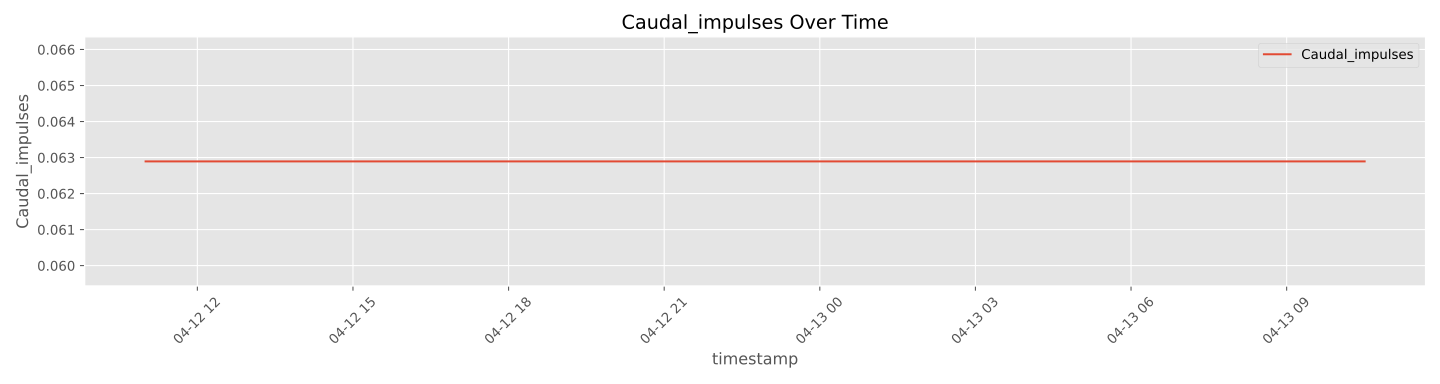
\includegraphics[width=\textwidth]{Caudal_impulses.png}
        \caption*{Caudal Impulses}
    \end{minipage}
    \hfill
    \begin{minipage}[b]{0.45\textwidth}
        \centering
        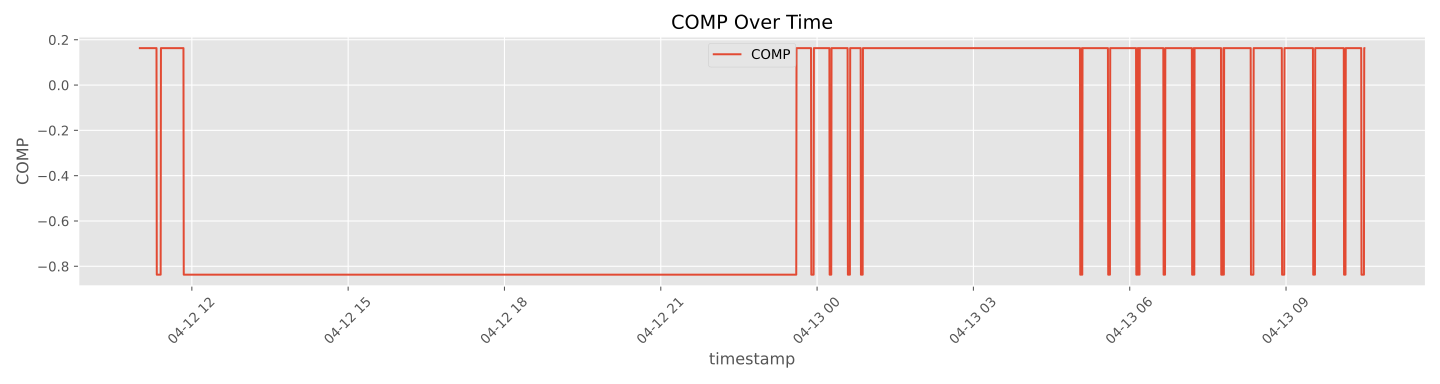
\includegraphics[width=\textwidth]{COMP.png}
        \caption*{COMP}
    \end{minipage}
    \vspace{0.5em} % Adds space between rows

    \begin{minipage}[b]{0.45\textwidth}
        \centering
        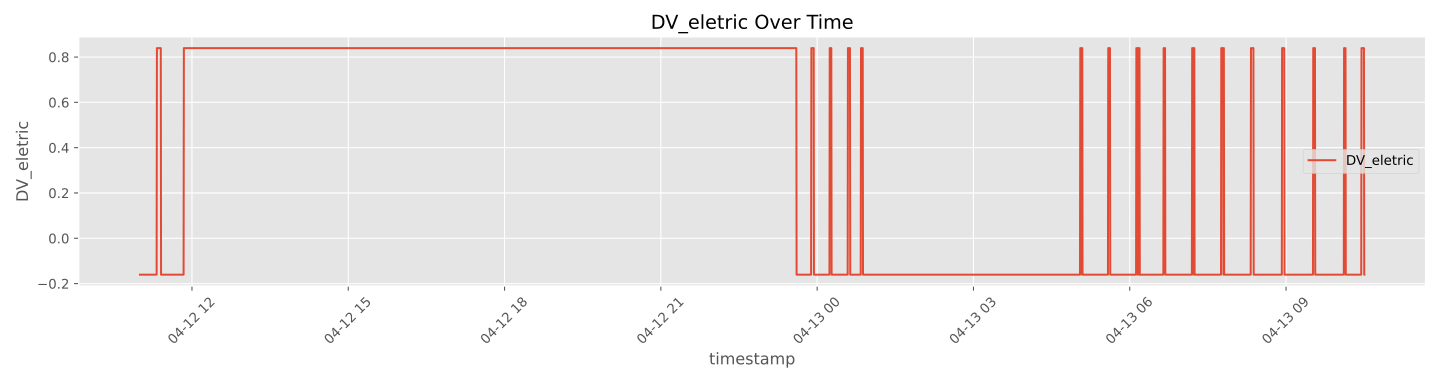
\includegraphics[width=\textwidth]{DV_eletric.png}
        \caption*{DV Electric}
    \end{minipage}
    \hfill
    \begin{minipage}[b]{0.45\textwidth}
        \centering
        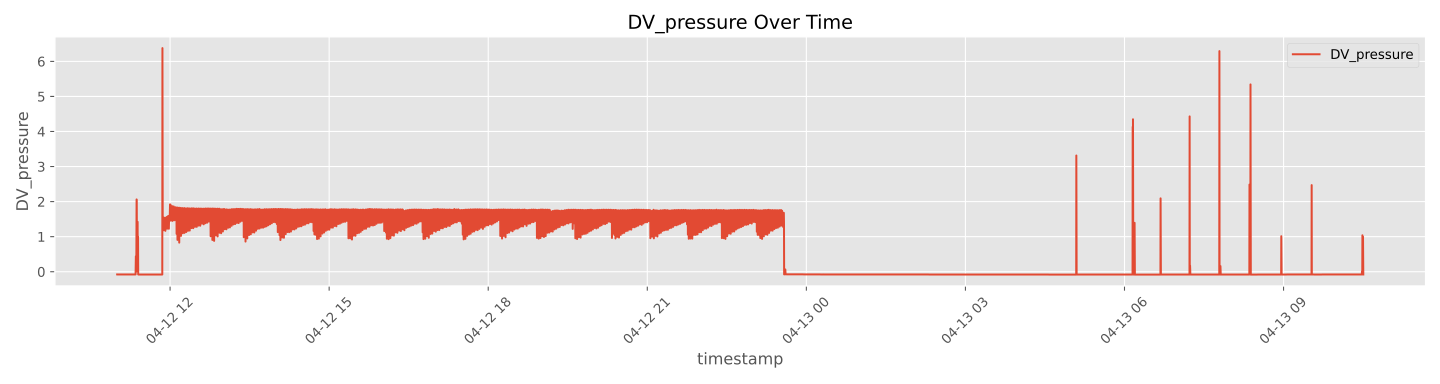
\includegraphics[width=\textwidth]{DV_pressure.png}
        \caption*{DV Pressure}
    \end{minipage}
    \vspace{0.5em}

    \begin{minipage}[b]{0.45\textwidth}
        \centering
        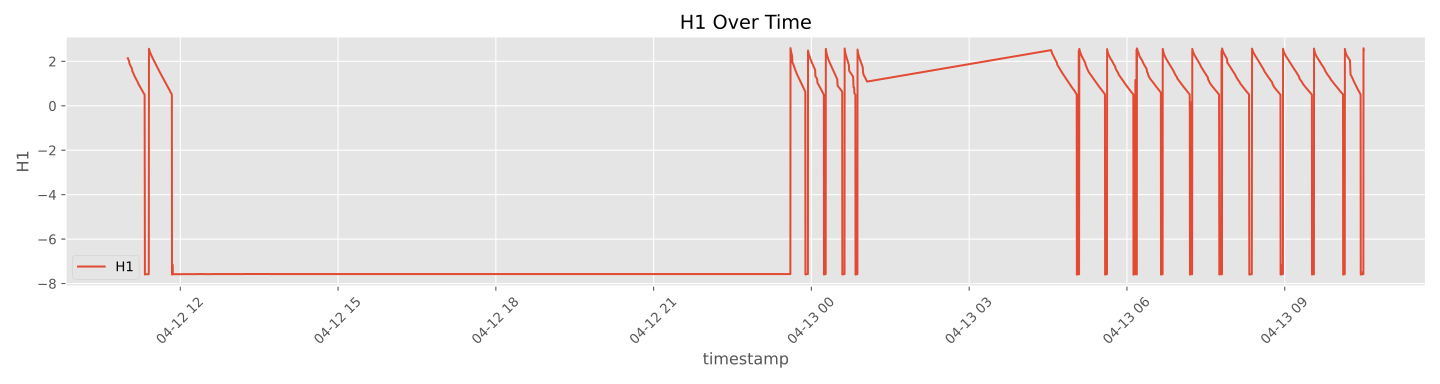
\includegraphics[width=\textwidth]{H1.png}
        \caption*{H1}
    \end{minipage}
    \hfill
    \begin{minipage}[b]{0.45\textwidth}
        \centering
        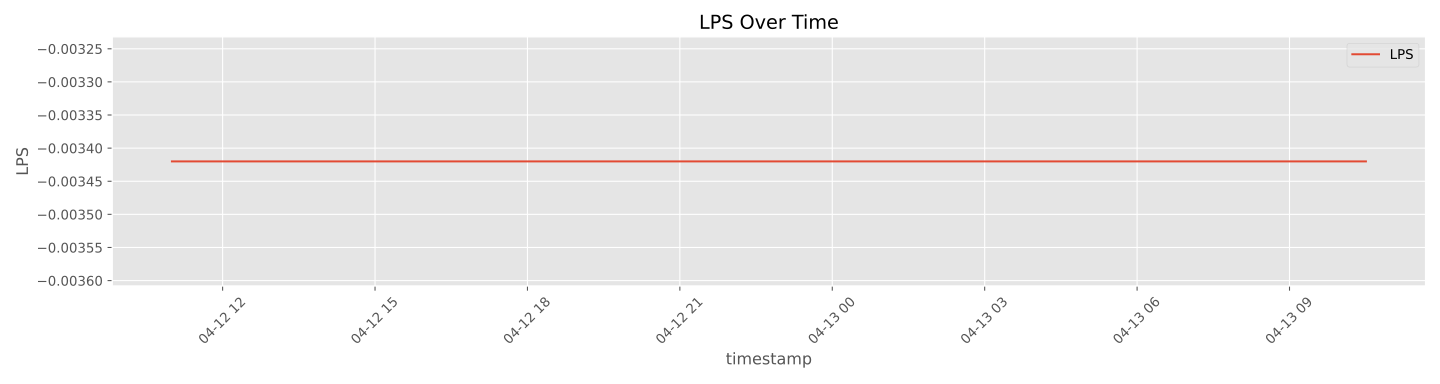
\includegraphics[width=\textwidth]{LPS.png}
        \caption*{LPS}
    \end{minipage}
    \vspace{0.5em}

    \begin{minipage}[b]{0.45\textwidth}
        \centering
        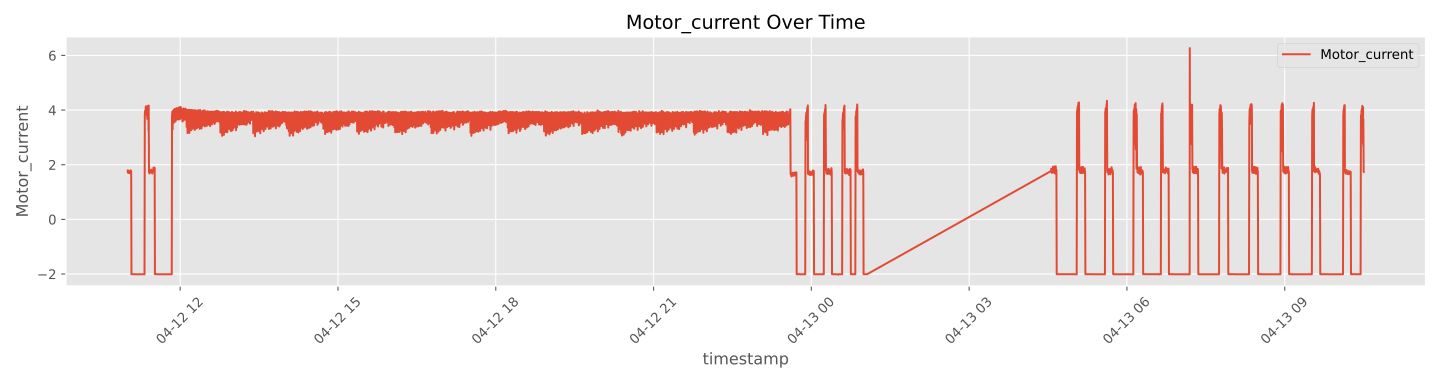
\includegraphics[width=\textwidth]{Motor_current.png}
        \caption*{Motor Current}
    \end{minipage}
    \hfill
    \begin{minipage}[b]{0.45\textwidth}
        \centering
        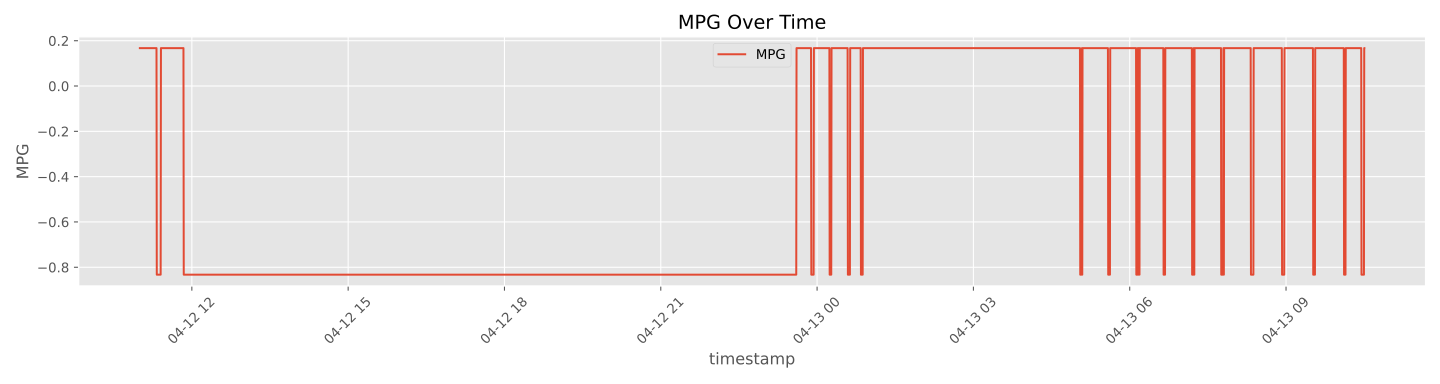
\includegraphics[width=\textwidth]{MPG.png}
        \caption*{MPG}
    \end{minipage}
    \vspace{0.5em}

    \begin{minipage}[b]{0.45\textwidth}
        \centering
        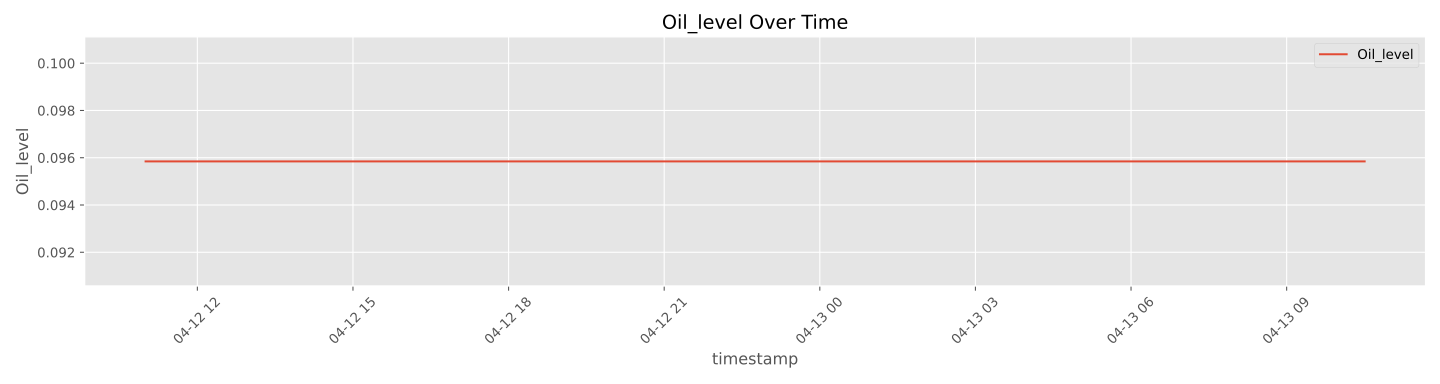
\includegraphics[width=\textwidth]{Oil_level.png}
        \caption*{Oil level}
    \end{minipage}
    \hfill
    \begin{minipage}[b]{0.45\textwidth}
        \centering
        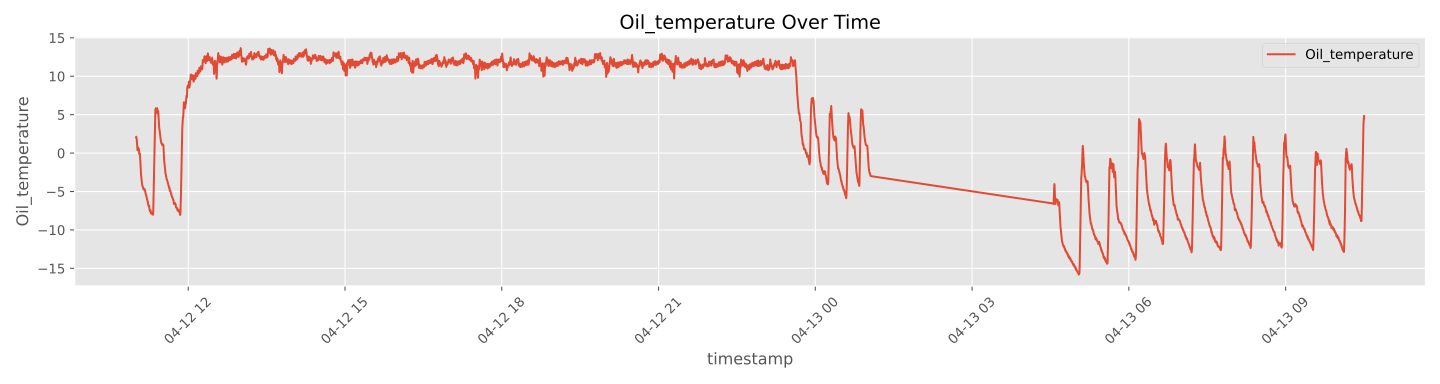
\includegraphics[width=\textwidth]{Oil_temperature.png}
        \caption*{Oil temperature}
    \end{minipage}
    \vspace{0.5em}

    \begin{minipage}[b]{0.45\textwidth}
        \centering
        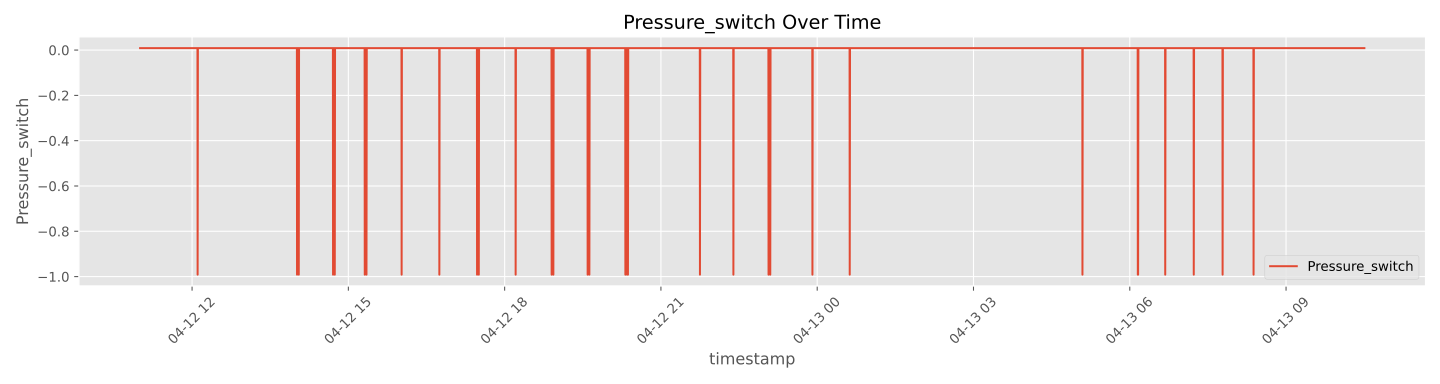
\includegraphics[width=\textwidth]{Pressure_switch.png}
        \caption*{Pressure switch}
    \end{minipage}
    \hfill
    \begin{minipage}[b]{0.45\textwidth}
        \centering
        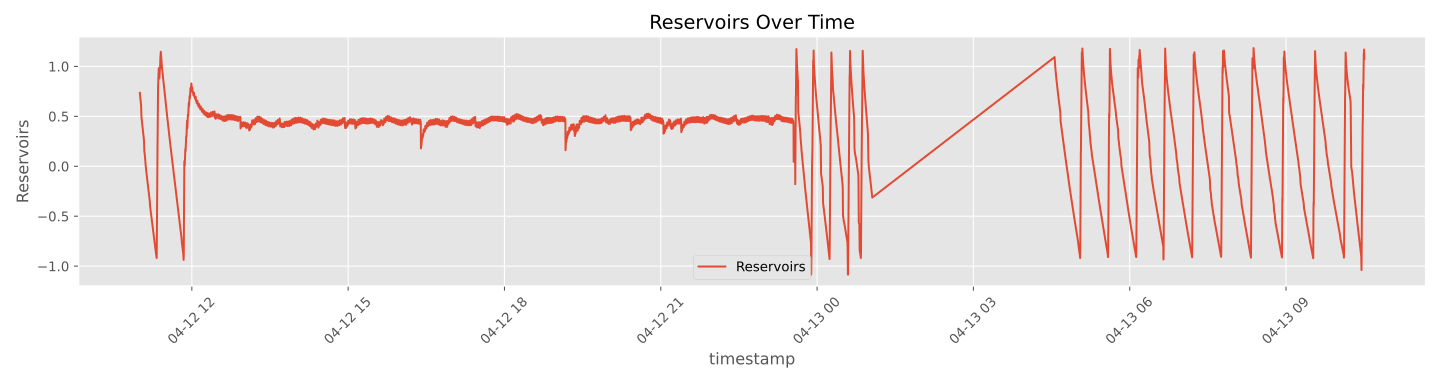
\includegraphics[width=\textwidth]{Reservoirs.png}
        \caption*{Reservoirs}
    \end{minipage}
\caption{Variables en rangos donde hay anomalías. Se observa cambios bruscos en la naturaleza cíclica del uso habitual del motor de compresión.}
\label{fig:anomaly_in_variables}
\end{figure}

\begin{figure}[htp]
    \centering
    \vspace{0.5em}

    \begin{minipage}[b]{0.45\textwidth}
        \centering
        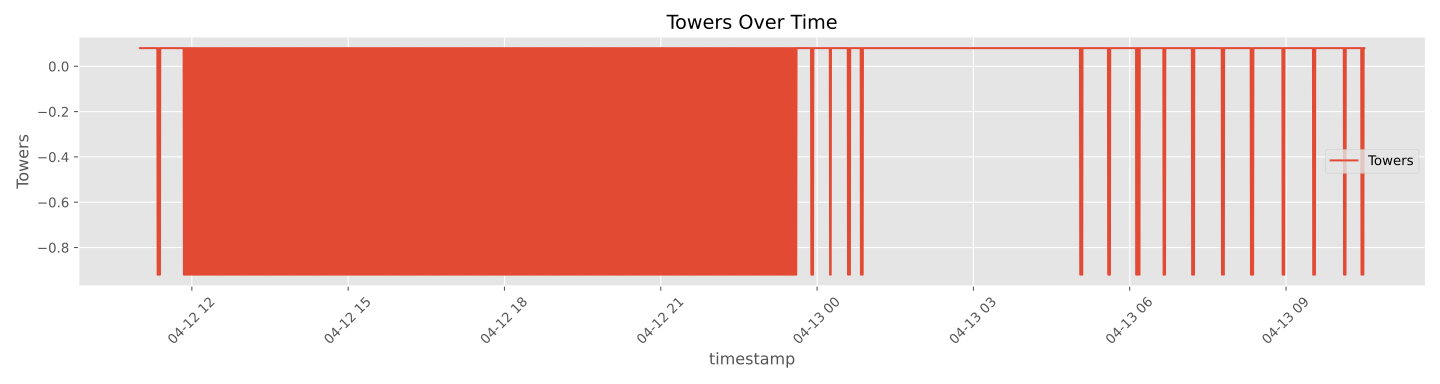
\includegraphics[width=\textwidth]{Towers.png}
        \caption*{Towers}
    \end{minipage}
    \hfill
    \begin{minipage}[b]{0.45\textwidth}
        \centering
        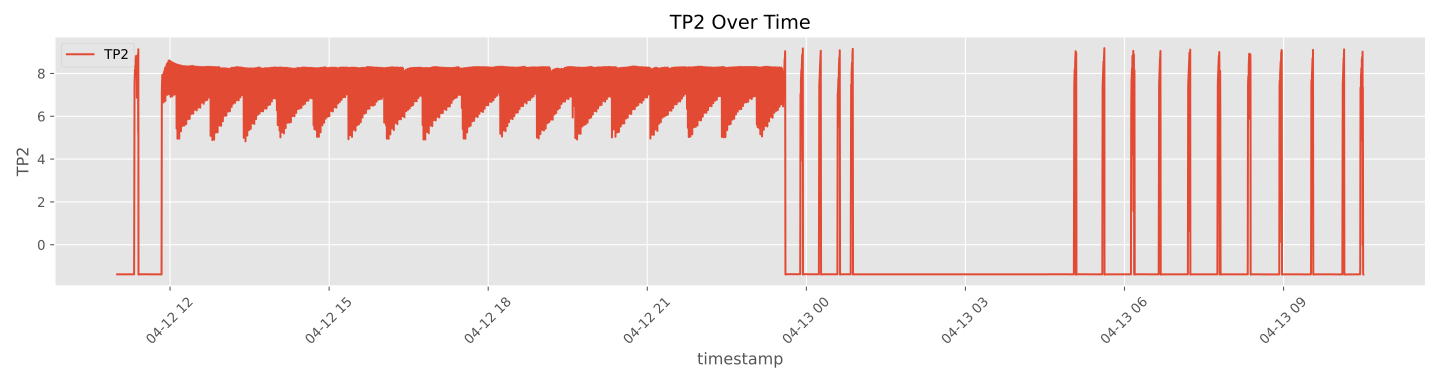
\includegraphics[width=\textwidth]{TP2.png}
        \caption*{TP2}
    \end{minipage}
    \vspace{0.5em}

    \begin{minipage}[b]{0.45\textwidth}
        \centering
        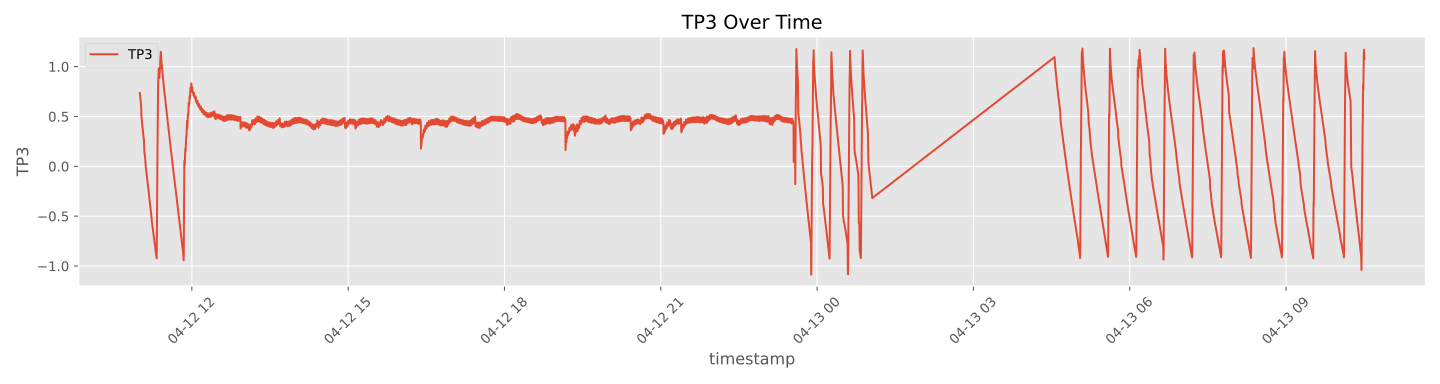
\includegraphics[width=\textwidth]{TP3.png}
        \caption*{TP3}
    \end{minipage}

    \caption{Variables en rangos donde hay anomalías.}
    \label{fig:anomaly_in_variables2}
\end{figure}

Como puede observarse en la Figura~\ref{fig:anomaly_in_variables} y en la Figura~\ref{fig:anomaly_in_variables2}, se visualizan los rangos donde según expertos, se produjo una anomalía. Gracias a esto es posible observar con facilidad que tipo de forma toma cada variable cuando una anomalía ocurre.

\begin{figure}[htp]
    \centering
    \subfloat{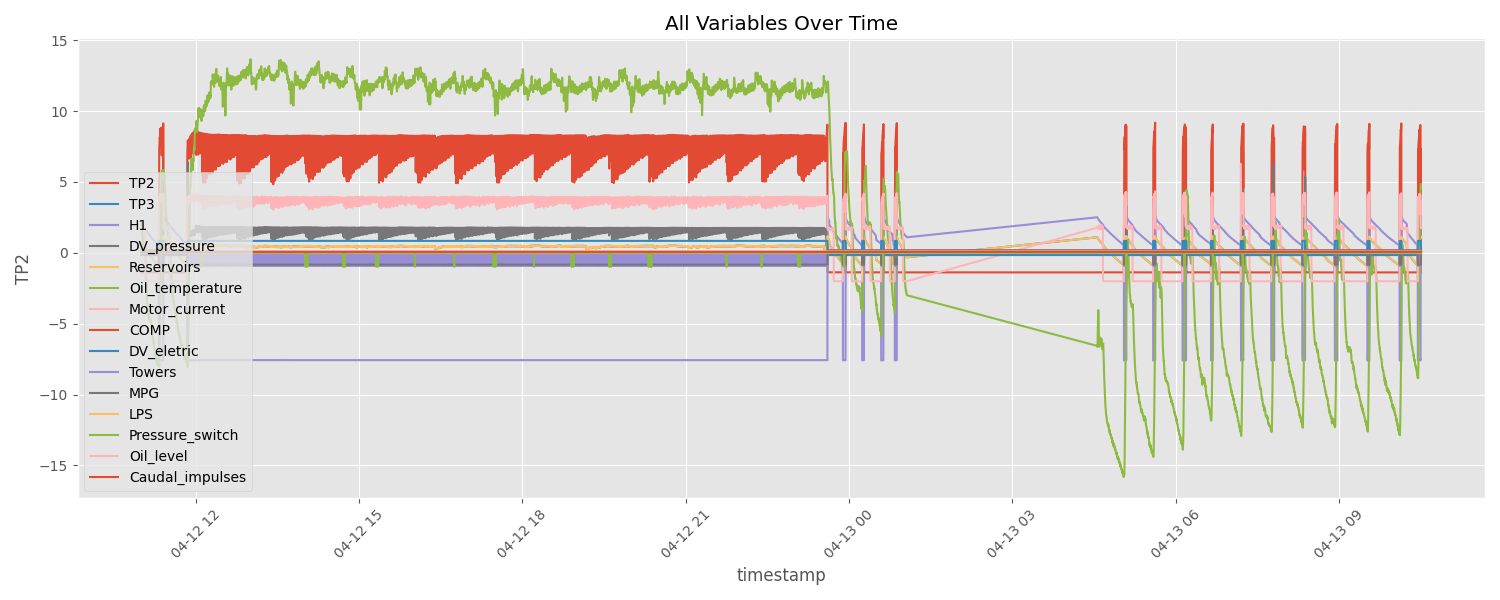
\includegraphics[width=0.7\textwidth]{all_anomalies.png}}
    \caption{Todas las variables en funcionamiento normal y durante anomalías. }
    \label{fig:all_anomalies}
\end{figure}

En la Figura~\ref{fig:all_anomalies} se muestran todas las anomalías (centradas gracias al estandarizado sobre la media) y cómo se comportan en un rango anómalo. Se preserva la varianza de cada una de ellas de forma que pueda observarse su rango de valores completo real.

\begin{figure}[htp]
    \centering
    \subfloat{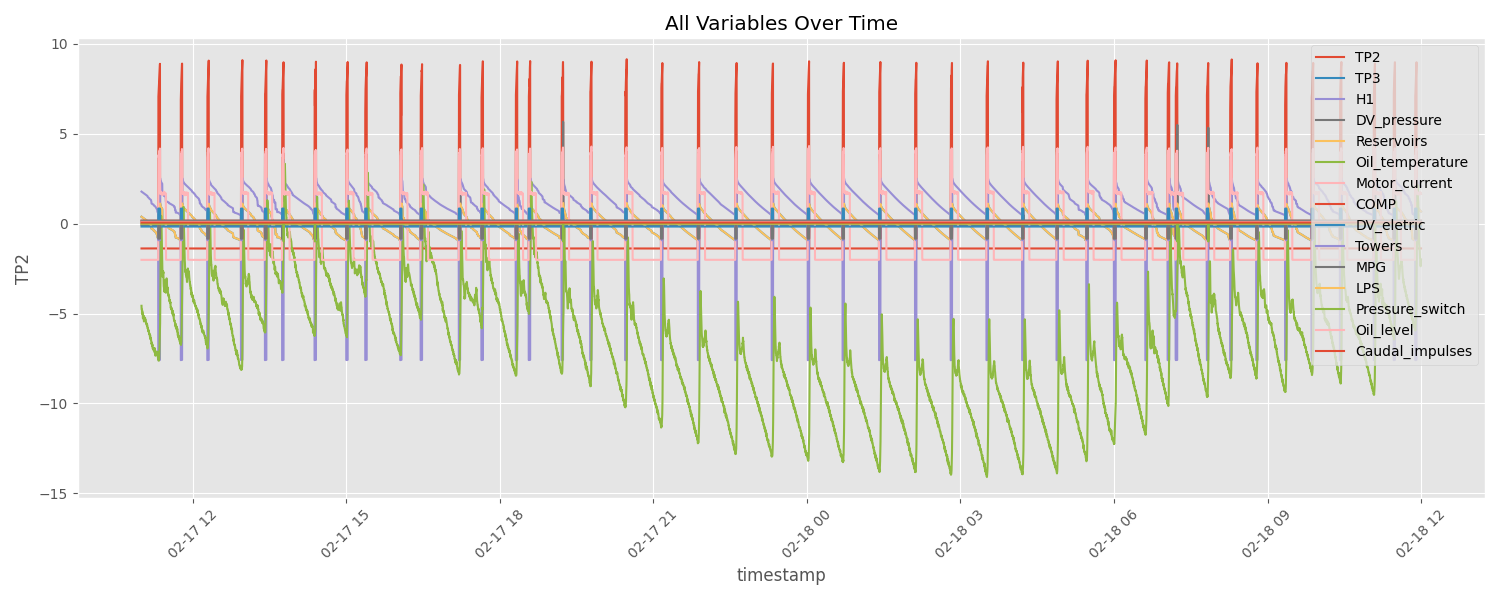
\includegraphics[width=0.7\textwidth]{all_normal.png}}
    \caption{Todas las variables en rangos normales. Se observa la naturaleza cíclica de todas las variables debido a que iteraccionan en conjunto.}
    \label{fig:all_normal}
\end{figure}


Si se muestra otro rango temporal, se puede observar el comportamiento esperado de cada variable. De hecho, se podría intuir que son series de naturaleza \textbf{estacionaria}. Este fenómeno puede observarse en la Figura~\ref{fig:all_normal}.
Una serie estacionaria es una secuencia de datos temporales cuyas propiedades estadísticas, como la media, la varianza y la autocorrelación, son constantes a lo largo del tiempo. Esto significa que su comportamiento no cambia dependiendo del momento en el que se analice, lo que facilita su modelado y predicción.

\subsection{Test estadísticos}
Se realizan pruebas estadísticas a las series temporales con el objetivo de determinar si son estacionarias. En este contexto, si el valor crítico de la prueba es mayor que el valor estadístico obtenido, se concluye que la serie no es estacionaria.
Entre las pruebas utilizadas, destaca la prueba de \textit{Dickey-Fuller Aumentada} (ADF), un test estadístico diseñado para evaluar la presencia de una raíz unitaria en una serie temporal. La existencia de una raíz unitaria indica que la serie no es estacionaria.

Ya que se tienen muchos datos, hacer la prueba de \textit{adfuller} con todos en cada columna no es viable. Por tanto, de manera aleatoria se escogen muestras de tramos aleatorios de cada variable. De esta manera se puede evaluar si la serie es estacionaria en gran parte de sus tramos y deducir si la serie completa es posible que sea estacionaria (veáse la Tabla~\ref{tab:stationary_results}).

\begin{table}[htp]
    \centering
    \begin{tabular}{lcccc}
    \hline
    Variable & Repeticiones & Promedio del test & p-valor promedio & ¿Es estacionaria? \\
    \hline
    TP3 & 9/10 & -5.32 & $10^{-4}$ & Sí \\
    H1 & 10/10 & -6.24 & $10^{-7}$ & Sí \\
    DV eletric & 8/10 & -5.68 & $10^{-6}$ & Sí \\
    DV pressure & 9/10 & -21.32 & $10^{-22}$ & Sí \\
    Caudal impulses & 0/10 & - & - & Valor Contante \\
    TP2 & 9/10 & -6.29 & $10^{-7}$ & Sí \\
    Pressure switch & 9/10 & -20.91 & $10^{-13}$ & Sí \\
    Reservoirs & 10/10 & -5.68 & $10^{-6}$ & Sí \\
    Towers & 10/10 & -6.81 & $10^{-9}$ & Sí \\
    LPS & 1/10 & -4.76 & $10^{-5}$ & Parcialmente \\
    Oil level & 2/10 & -2.59 & $0.1$ & No \\
    COMP & 10/10 & -5.99 & $10^{-6}$ & Sí \\
    Motor current & 9/10 & -4.56 & $10^{-4}$ & Sí \\
    MPG & 9/10 & -6.09 & $10^{-7}$ & Sí \\
    Oil temperature & 10/10 & -5.28 & $10^{-5}$ & Sí \\
    \hline
    \end{tabular}
    \caption{Tabla de resultados tras $10$ repeticiones en tramos aleatorios}
    \label{tab:stationary_results}
\end{table}


\subsection{Preprocesamiento}

\subsubsection{Enfoques del problema}


Existen dos enfoques principales para abordar el estudio de este problema, los cuales varían dependiendo de si se incorporan o no valores temporales. El \textbf{primer enfoque} se basa en el uso de \textbf{instantáneas} y prescinde de la información temporal. En este enfoque, en cada iteración, los sensores del compresor generan un vector de valores representativos del estado del sistema en ese momento específico. Este vector se puede utilizar para predecir la presencia de posibles anomalías en el compresor, sin considerar las variaciones temporales previas.

Este método tiene la ventaja de permitir una detección rápida de anomalías, ya que, si es capaz de identificar correctamente los fallos, proporcionaría una respuesta con el menor retardo posible, e incluso en tiempo real. La ventaja principal de este enfoque radica en su simplicidad y capacidad de ofrecer una alerta inmediata ante cualquier fallo en el compresor, lo que resulta crucial en aplicaciones donde la rapidez en la respuesta es fundamental.

El \textbf{segundo enfoque} se basa en la \textbf{incorporación de información temporal} y utiliza valores dentro de una ventana de tiempo determinada para identificar posibles fallos en el compresor. A través de este enfoque, el modelo encargado de la detección de anomalías es capaz de realizar un análisis más detallado de las tendencias a lo largo del tiempo. Este análisis temporal permite captar patrones que, de otro modo, podrían pasar desapercibidos al considerar únicamente instantáneas.

Es razonable suponer que ciertos fallos no se manifiestan mediante cambios abruptos en los valores de los sensores, sino que se desarrollan progresivamente. Por ejemplo, una disminución gradual del nivel de aceite, que ocurre a una velocidad mayor de la esperada, podría ser suficiente para señalar el inicio de un fallo. En estos casos, el análisis de los valores temporales sería esencial, ya que permite detectar anomalías antes de que los valores de los sensores alcancen niveles extremos. Esto, en un contexto predictivo, posibilitaría adelantarse al fallo y, potencialmente, evitarlo.

No obstante, este enfoque no está exento de desafíos. Una de las principales limitaciones es que los valores anómalos pueden quedar ``opacados'' o diluidos por el resto de los datos dentro de la ventana temporal, lo que podría dificultar la identificación precisa de anomalías. Sin embargo, el equipo considera que la información temporal ofrece una ventaja significativa en la detección temprana de fallos, por lo que ha decidido centrar su trabajo en este enfoque. A continuación, se abordarán con mayor detalle las características de este modelo y cómo se gestionan los posibles problemas derivados de la utilización de información temporal en el proceso de detección.

\subsubsection{Definición de la ventana deslizante}

Para resolver este problema estudiamos los tiempos de activaciones de los motores para poder definir una ventana deslizante que pueda recoger información de la activación de los mismos. 
Para ello, se ha calculado la mediana del tiempo de activación de los motores. Para ello, se ha detectado la activación y apagado del motor por medio de la variable ``\textit{Motor current}'', cuyos 
valores para apagado son inferiores a 0.05, veáse la Figura~\ref{fig:VisualizacionDatos}.

\begin{figure}[htp]
        \centering
        \subfloat{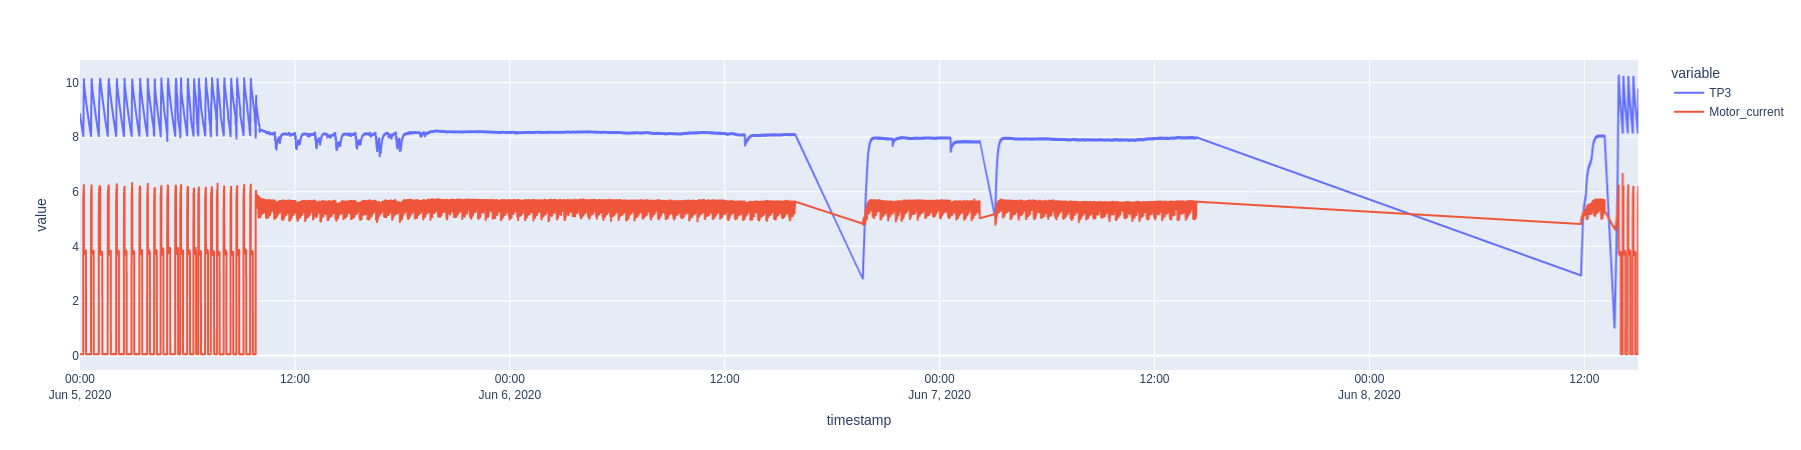
\includegraphics[width=0.7\textwidth]{VisualizacionDatos.png}}
        \caption{Observamos los datos y los valores de la presión en el panel neumático (TP3, línea azul) y la corriente del motor (línea roja).}
        \label{fig:VisualizacionDatos}
\end{figure}

Se han recogido los resultados en la Tabla~\ref{tab:TiempoCiclo}. La mediana se calcula sobre los intervalos de tiempo no anómalos. No obstante, 
aunque el conjunto de datos no presenta valores pérdidos en ninguna de las columnas, sí que presenta saltos temporales. Los datos de los sensores se mostrean cada 10 segundos, 
pero se ha encontrado saltos temporales de incluso días, véase Figura~\ref{fig:VentanaDeslizante}. Se planteó la posibilidad de interpolar los datos, pero dada la naturaleza 
del problema, serie temporal pseudo-cíclica pero con intervalos distintos, es difícil obtener resultados prometedores para saltos grandes sin la posibilidad de ``ensuciar'' la calidad de los datos.
Por ello, se ha calculado el tiempo mediano de ciclo de motor tras eliminar los saltos temporales. Para comprobar, se ha calculado también la mediana 
para todos intervalos sin anomalías de la Tabla~\ref{tab:Reportes}. Los valores obtenidos están muy cerca del especificado en la Tabla~\ref{tab:TiempoCiclo}.

\begin{table}[htp]
    \centering
    \begin{tabular}{c}
    \hline
    \textbf{Mediana del tiempo de ciclo} \\ \hline 
    1260 segundos\\
    \hline
    \end{tabular}
    \caption{Resultado obtenido del cálculo de la ventana deslizante. Se acerca a los obtenidos en el artículo original de detección de fallos de este dataset~\cite{FailureDetection}.}
    \label{tab:TiempoCiclo}
\end{table}

Para la asignación de los grupos se ha utilizado dos veces la mediana del tiempo de ciclo del motor. 
Esto es debido a que así se puede asegurar contener información de almenos más de la mitad de la activación del motor, asegurando que predecimos con la mayor información posible del estado del motor.
Se puede observar la asignación de grupos en la Figura~\ref{fig:VentanaDeslizante}.

\begin{figure}[htp]
        \centering
        \subfloat{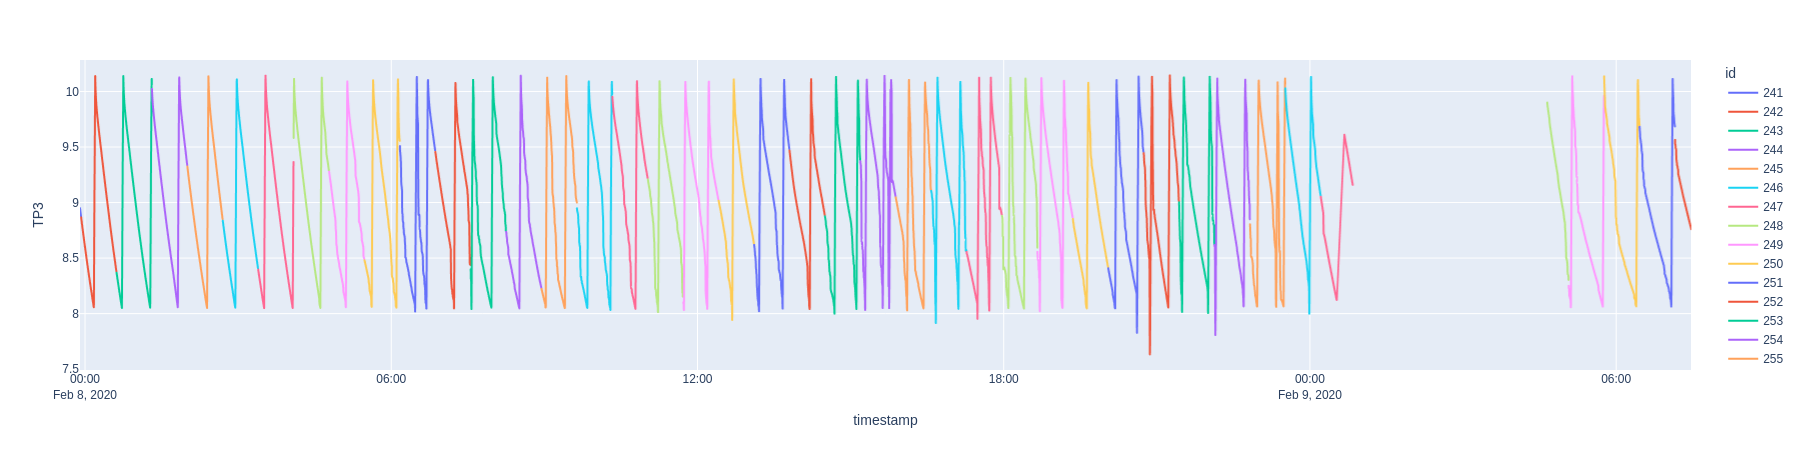
\includegraphics[width=0.7\textwidth]{VentanaDeslizante.png}}
        \caption{Observamos los grupos asignados de utilizar 2 veces el tiempo de ciclo.}
        \label{fig:VentanaDeslizante}
\end{figure}


Durante el análisis EDA y prepración del conjunto de datos de entrenamiento y evaluación se han recogido nuevas anomalías, veáse la Tabla~\ref{tab:EventosRaros} y Figura~\ref{fig:EventosRaros}.
Sería interesante volver a consultar con un experto del campo para que valide dichas anomalías. No obstante, presentan un perfil suficientemente cercano al de las anomalías clasificadas.
Por ello, consideramos oportuno la inclusión de dichos ejemplos como anomalías para ayudar a resolver el problema del bajo número de ejemplo de casos positivos.

\begin{table}[htp]
    \centering
    \begin{tabular}{cllrl}
    \hline
    \textbf{Número} & \textbf{Inicio}       & \textbf{Fin}         & \textbf{Duración (min)} & \textbf{Importancia} \\ \hline
    22 & 2020-03-06 21:42:15 & 2020-03-06 23:14:00 & 92 & - \\ 
    23 & 2020-03-11 05:15:10 & 2020-03-11 06:25:00 & 70 & - \\ 
    24 & 2020-03-12 00:15:56 & 2020-03-12 11:59:00 & 704 & - \\
    25 & 2020-03-26 04:00:20 & 2020-03-26 05:20:00 & 80 & - \\ 
    26 & 2020-03-27 07:12:00 & 2020-03-27 12:01:00 & 289 & - \\
    27 & 2020-04-17 08:50:28 & 2020-04-17 23:59:00 & 909 & - \\
    28 & 2020-04-25 00:07:15 & 2020-04-25 01:10:00 & 63 & - \\ 
    29 & 2020-05-19 01:35:28 & 2020-05-19 02:40:00 & 64 & - \\ 
    30 & 2020-06-12 01:41:07 & 2020-06-12 17:06:00 & 925 & - \\
    31 & 2020-07-21 13:32:48 & 2020-07-21 22:03:00 & 510 & - \\
    32 & 2020-07-22 06:40:46 & 2020-07-22 13:10:00 & 389 & - \\
    33 & 2020-07-31 00:57:33 & 2020-07-31 02:09:00 & 71 & - \\ \hline
    \end{tabular}
    \caption{Intervalos de tiempo encontrados con valores constantes y fluctuaciones extrañas, un patrón similar al de las anomalías, sin etiquetado.}
    \label{tab:EventosRaros}
\end{table}

\begin{figure}[htp]
        \centering
        \subfloat{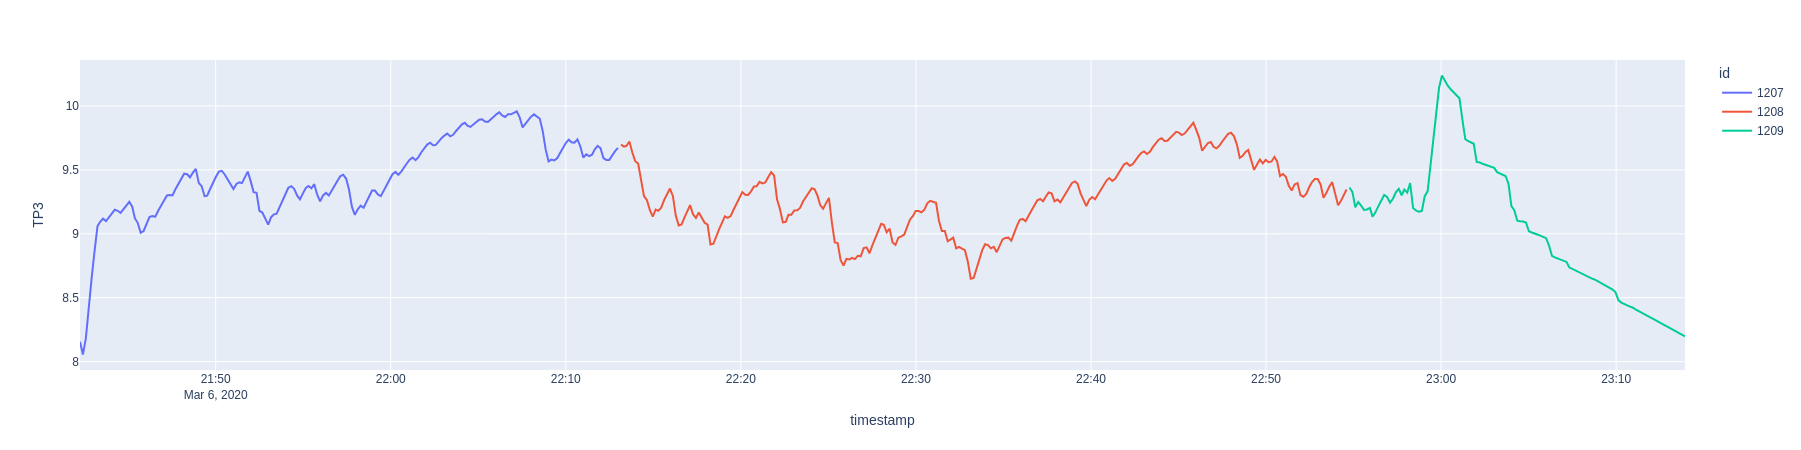
\includegraphics[width=0.7\textwidth]{EjemploRaro1.png}}\\
        \subfloat{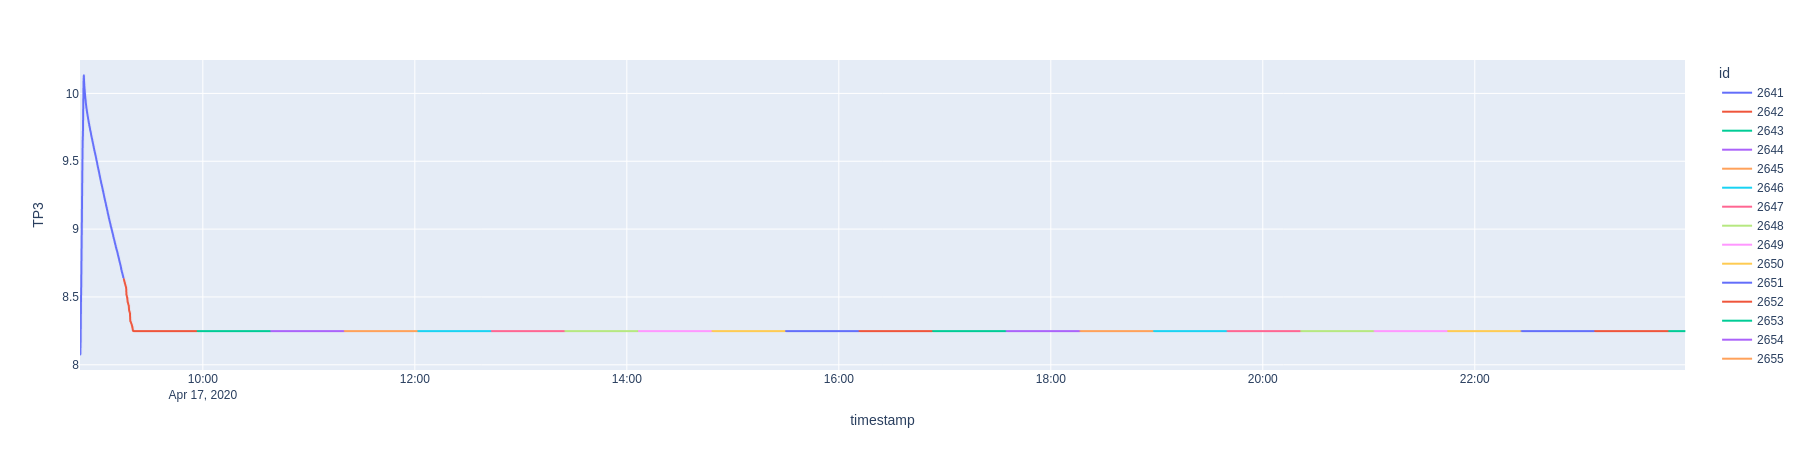
\includegraphics[width=0.7\textwidth]{EjemploRaro2.png}}
        \caption{Ejemplo de nuevos intervalos anómalos encontrados. Observamos valores constantes o fluctuaciones fuera de lo habitual para el motor apagado o encendido.}
        \label{fig:EventosRaros}
\end{figure}

Tras observar y analizar el conjunto de datos, seguimos un acercamiento similar a~\cite{PredictiveMaintenance,FailureDetection} para tratar a la serie temporal, 
se ha optado por la transformación de los intervalos de las ventanas deslizante en obtener el promedio, mínimo, máximo y varianza de cada variable durante el intervalo de tiempo mostreado. 
Para resolver el problema de saltos temporales, se ha eliminado aquellos conjuntos en los que se estiman estas variables para un número de puntos inferior a $(\textrm{tiempo de ciclo}) / 10 = 126$. Ya que esos ejemplos 
son estimados con menos puntos que el tiempo de activación del motor, lo cuál puede generar estimaciones del promedio y varianza sub-óptimos.

\subsubsection{Generación de conjuntos}

Una vez determinado la ventana deslizante y las características a extraer, se genera las diferentes instancias y se divide en los conjuntos de entrenamiento y evaluación. Se debe determinar por tanto si un intervalo de la ventana deslizante es una anomalía o no, para lo cuál es utilizado se utilizado un criterio de votación en el cuál gana la mayoría.

Uno de los aspectos cruciales a considerar en este enfoque es la similitud de los datos generada por la ventana deslizante en ciertos momentos. Por ejemplo, en el caso de anomalías cuya duración se extiende por un periodo de tiempo considerable, como un día completo (por ejemplo, de 6/05/2020 10:00 a 6/05/2020 23:59), se generan ventanas de 21 minutos en cada iteración. Esto puede dar lugar a la aparición de instantes temporalmente muy similares entre sí, lo que podría influir en la evaluación de los modelos de detección de anomalías.

Una situación problemática podría ocurrir si las ventanas se distribuyeran de manera completamente aleatoria a posteriori. En ese caso, se podría dar el escenario en el cual un periodo como \textbf{6/05/2020 10:00 - 6/05/2020 10:21} pertenezca al conjunto de entrenamiento, mientras que el siguiente periodo \textbf{6/05/2020 10:21 - 6/05/2020 10:42} esté en el conjunto de test. Esta división podría generar evaluaciones poco representativas, ya que las ventanas de tiempo consecutivas podrían estar separadas en diferentes conjuntos de datos, lo que afectaría la validez de la evaluación de la capacidad predictiva del modelo. Véase la figura \ref{fig:VentanaDeslizante}.

\begin{figure}[htp]
        \centering
        \subfloat{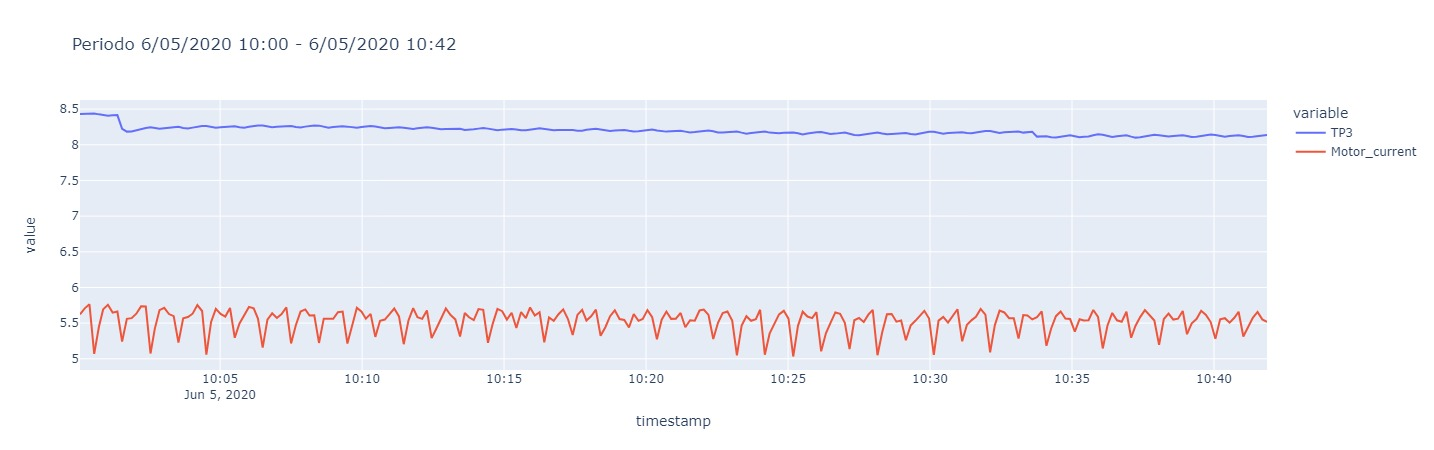
\includegraphics[width=0.7\textwidth]{prueba_agrupacion.jpeg}}
        \caption{Observamos la similitud de los valores de algunos sensores durante la anomalía.}
        \label{fig:PruebaAgrupacion}
\end{figure}

Para mitigar este riesgo y garantizar una evaluación más precisa y coherente, las instancias se agrupan temporalmente. De esta forma, se asegura que dos instancias pertenecientes al mismo grupo no se distribuyan entre los conjuntos de entrenamiento y test si dichos conjuntos se utilizan con fines de validación y entrenamiento. Se define un \textbf{grupo} como un conjunto de ventanas que comparten el mismo tipo (anomalía o no anomalía) y no presentan saltos temporales, es decir, no existe un periodo sin datos entre las ventanas. Este enfoque asegura que la información utilizada en el entrenamiento y la validación sea coherente y representativa, mejorando así la robustez de las evaluaciones del modelo.

El proceso de generación de los conjuntos de datos consiste en barajar los grupos de ventanas deslizantes para asignar de forma aleatoria diferentes grupos de intervalos de tiempo en cada partición, 
evitando así pliegues más fáciles o difíciles (obtener unos resultados más balanceados en general). Es decir, agrupamos los grupos en grupos de mayor tamaño, pero esta vez mediante la aleatoriedad y teniendo en cuanta la proporción de grupos anómalos y grupos no anómalos.

Concretamente, se decide dividir los datos en 9 pliegues. Se estima el número de anomalías que pertenecería a cada pliegue y se genera conjuntos lo más equilibrado posible (véase la Tabla~\ref{tab:ValidacionCruzada}). 
Por último, se asigna el pliegue 1 y 8 (elección aleatoria) como el conjunto de test. Los resultantes serán agrupado en 4 pliegues para el entrenamiento de la validación cruzada. 

\begin{table}[htp]
    \centering
    \begin{tabular}{cccc}
    \hline
    \textbf{Pliegue} & \textbf{Negativo} & \textbf{Positivo} & \textbf{Conjunto}\\ \hline
        0 & 635 & 31 & Evaluación \\ 
        1 & 635 & 31 & Etrenamiento pliegue 1 \\ 
        2 & 635 & 31 & Etrenamiento pliegue 2\\ 
        3 & 635 & 31 & Etrenamiento pliegue 3\\ 
        4 & 635 & 31 & Etrenamiento pliegue 4\\ 
        5 & 635 & 31 & Etrenamiento pliegue 3\\ 
        6 & 635 & 31 & Etrenamiento pliegue 2 \\
        7 & 638 & 31 & Etrenamiento pliegue 1\\ 
        8 & 641 & 43 & Evaluación \\ \hline
    \end{tabular}
    \caption{Distribución de los 9 pliegues generados. Se asigna de forma aleatoria el 1 y 8 a test. Se agrupan los demás hasta forma 4 pliegues usando el primer y último de los restantes: 0 y 7, 2 y 6, 5 y 3, 4.}
    \label{tab:ValidacionCruzada}
\end{table}

\section{Métricas de evaluación}\label{sec:Metricas}

Debido a que tratamos de evaluar el rendimiento de diferentes modelos para la resolución de un problema de detección de anomalías, 
el uso de métricas como la \textbf{precisión}, la \textbf{sensibilidad} (\textit{recall}) y la \textbf{puntuación F1} es fundamental para evitar evaluaciones sesgadas. 
Cada una de estas métricas aporta una perspectiva única sobre cómo el modelo maneja tanto las clases mayoritarias (no anomalías) como las minoritarias (anomalías).

\begin{itemize}
    \item \textbf{Precisión}: mide la proporción de verdaderos positivos entre todas las instancias clasificadas como positivas. Esto permite evaluar qué tan confiable es el modelo al detectar anomalías sin producir demasiados falsos positivos.
    \item \textbf{Sensibilidad}: evalúa la capacidad del modelo para identificar correctamente todas las anomalías presentes en el conjunto de datos. Esta métrica es crucial en aplicaciones donde no detectar una anomalía puede tener consecuencias graves.
    \item \textbf{F1}: como métrica armonizada entre precisión y sensibilidad, es especialmente útil en tareas de detección de anomalías, ya que equilibra ambos aspectos, permitiendo evaluar el rendimiento del modelo en contextos donde el costo de los falsos positivos y falsos negativos debe ser considerado conjuntamente.
\end{itemize}

Es por ello que en las diferentes experimentaciones se ha hecho uso de esas métricas. La evaluación es el promedio del rendimiento de los modelos en los diferentes pliegues de validación. 

\section{Máquinas de Vectores de Soporte (Ana Fuentes)}
A continuación, se ha implementado un modelo SVM (Support Vector Machine) para trabajar con los conjuntos de datos de entrenamiento y test. Este modelo es eficaz para problemas de clasificación binaria con relaciones no lineales, especialmente cuando el número de características es elevado, como ocurre en este caso.\\
Antes de construir este modelo, se han escalado los datasets de entrenamiento y de test aplicando la función \texttt{StandardScaler} para normalizar los datos, lo que es crucial en modelos como SVM, que son sensibles a la magnitud de las características. Seguidamente, se ha implementado la función \texttt{get\_cv\_iterable} para obtener las cuatro separaciones del conjunto de entrenamiento para poder hacer la validación cruzada. Con estos pequeños ajustes, se ha procedido a la configuración del modelo básico de SVM. \\

En primer lugar, se han ajustado los siguientes hiperparámetros:
\begin{itemize}
    \item C: este parámetro controla la penalización por errores de clasificación.
    \item $\gamma$: este define cómo influye una sola muestra en el modelo, lo que resulta relevante para kernels no lineales.
    \item Kernel: también se elige entre dos tipos de kernel, ``rbf'' o ``linear''.
\end{itemize}

Tras la inicialización de estos parámetros, se ha utilizado \texttt{GridSearchCV} para realizar una búsqueda exhaustiva de combinaciones de los hiperparámetros y se ha realizado la validación cruzada utilizando los folds predefinidos para evaluar cada combinación. De esta manera, se han probado 72 combinaciones, cuya mejor combinación ha resultado ser la mostrada en la Tabla \ref{tab:hiper-SVM}.
\begin{table}[H]
    \centering
    \begin{tabular}{ccc}
     \hline
     \textbf{C} & $\gamma$ & \textbf{kernel} \\ \hline
     10 & auto & rbf \\ \hline
    \end{tabular}
    \caption{Mejores hiperparámetros tras entrenar el modelo SVM.}
    \label{tab:hiper-SVM}
\end{table}

Una vez entrenado y obtenido el mejor modelo (como se pueder observar, se ha obtenido un kernel no lineal), se ha evaluado este modelo de SVM con el conjunto de prueba. Así pues, se han reflejado estos resultados en la Tabla \ref{tab:res-SVM}.
\begin{table}[H]
    \centering
    \begin{tabular}{ccccc}
    \hline
    \textbf{Clase} & \textbf{Precisión} & \textbf{Recall} & \textbf{F1-score} & \textbf{Soporte} \\ \hline
    False & 0.99 & 1.00 & 1.00 & 1279 \\ 
    True & 0.98 &  0.86 & 0.92 & 74 \\ 
    macro avg & 0.99 & 0.93 & 0.96 & 1353 \\ 
    weighted avg & 0.99 &  0.99 & 0.99 & 1353 \\ \hline
    \end{tabular}
    \caption{Resultados obtenidos de la evaluación del modelo SVM con el conjunto de prueba.}
    \label{tab:res-SVM}
\end{table}

Como se puede observar en esta Tabla, se han obtenido unos resultados deprecisión y recall para la clase ``False'' (no es anomalía) excelentes, lo que tiene sentido, al ser la mayoría de los datos no anómalos, ha aprendido mejor el modelo a identificar los valores que no son anomalías.\\
Por otro lado, la clase ``True'' (sí es anomalía) presenta un recall más bajo (86\%), lo que indica que 10 anomalías no fueron detectadas como tal.\\
A pesar de esto, el modelo alcanza un F1-score de 92\% en la clase ``True'', lo que refleja un buen balance entre precisión y recall.

Para finalizar, se ha generado la matriz de confusión que se puede observar en la Tabla \ref{tab:confusion-SVM}.
\begin{table}[H]
    \centering
    \begin{tabular}{|c|}
    \hline
    1278 \hspace{8mm} 1 \\ 
    10 \hspace{10mm} 64 \\ \hline
    \end{tabular}
    \caption{Matriz de confusión para el modelo implementado de SVM.}
    \label{tab:confusion-SVM}
\end{table}

En conclusión, el modelo SVM tiene un desempeño excelente con una precisión general del 99\%. Para la clase ``True'' presenta mayor dificultad de detección debido a la desbalanceada proporción entre las clases (muchos más datos no anómalos que anómalos).


\section{Clasificador Bayesiano (Brian Sena)}
El clasificador bayesiano (\textit{Naive Bayes}) es un algoritmo de clasificación basado en el Teorema de Bayes, el cual calcula la probabilidad posterior de una clase dado un conjunto de características de entrada. 
A pesar de su simplicidad, es una técnica poderosa y ampliamente utilizada en problemas de clasificación, como el filtrado de correos no deseados, la clasificación de textos y el análisis de sentimientos.
El modelo recibe el calificativo de ``\textit{naive}'' (ingenuo) debido a su principal asunción: \textbf{independencia condicional entre las características}, es decir, se supone que todas las variables predictoras son independientes entre sí dado el valor de la clase. 
Aunque esta asunción rara vez se cumple en escenarios del mundo real, \textit{Naive Bayes} sigue funcionando de manera sorprendentemente efectiva en muchos contextos, especialmente en dominios donde las relaciones entre variables no son complejas.

\subsection{Asunciones del Naive Bayes}
\begin{itemize}
    \item \textbf{Independencia condicional}: Se asume que las características son independientes entre sí. 
        En este caso, se asume que la variabilidad de una característica no depende del valor de otra. No obstante, ya vimos que los distintos sensores iteractúan entre sí, lo que hace débil a esta asunción.
    \item \textbf{Distribución de los datos:} \textit{Naive Bayes} asume que las características siguen una distribución normal dentro de cada clase. En nuestro caso, solamente se cumple para ``\textit{Pressure Switch}''.
    \item \textbf{Balance de clases}: El modelo puede ser sensible al desequilibrio de clases (cuando una clase es mucho más frecuente que otra), lo que puede sesgar las predicciones hacia la clase mayoritaria si no se toma en cuenta.
\end{itemize}

\subsection{Preprocesamiento}

Para implementar el \textit{Naive Bayes} de manera efectiva, es crucial preparar los datos adecuadamente. 
En este caso, no disponemos de variables categóricas que necesiten codificarse numéricamente ya que todas las características son numéricas y continuas. 
Además, se ha eliminado los saltos temporales y no se dispone de valores faltantes.
El algoritmo, dado que calcula distribuciones de probabilidad para cada clase~\cite{NaiveBayes} sin basarse en distancia, es invariante a la escala de los datos y, por ello, no necesitamos escalar los datos.
No obstante, aunque en el pre-procesamiento definido anteriormente se ha intentado crear un conjunto de datos equilibrado, disponemos de un drástico desequilibrio debido a la baja probabilidad de anomalía del sistema.
Es por ello que se ha incluído experimentación con métodos de submuestreo y sobremuestreo con técnicas como ``\textit{CondensedNearestNeighbour} (CNN)'' y ``\textit{SMOTE + TomekLinks} (SMOTETomek)''.
Por último, dado la primera asunción de independencia entre características se experimenta también con técnicas de selección de características, utilizando pruebas como la ``chi-cuadrado'' o ``información mutua''.

\subsection{Detalles de experimentación y resultados}\label{sec:ExpBayes}
En el caso de la experimentación con submuestreo o sobremuestreo se ha hecho uso de la librería ``\textit{imblearn}''~\cite{imblearn} y ``\textit{scikit-learn}''~\cite{sklearn}. 
La primera nos permite crear un \textit{pipeline} en el cuál solo se realiza las operaciones de submuestreo o sobremuestreo en los pliegues que correspondan al conjunto de entrenamiento en el bucle de validación. 
De esta forma, las estimaciones de la precisión no se veen afectado por estos cambios, permitiendo estimar mejor la capacidad de generalización del modelo. La segunda nos permite añadir otras operaciones si necesarias (por ejemplo una normalización) además de disponer de la implementación de los modelos.
Se ha realizado 4 pliegues de validación. Las métricas que utilizamos para evaluar el rendimiento se han discutido en la Sección~\ref{sec:Metricas}.
Para el clasificador bayesiano simples, el único hiperparámetro que tenemos que optimizar es el suavizado ($\alpha$) de la varianza para alargar la distribución de probabilidad de las clases.
Experimentaremos con los valores espaciados linealmente desde $1e^{-11 }$ a $1e^{-7}$ con 25 valores.

\begin{table}[!ht]
    \centering
    \begin{tabular}{llc}
        \hline
        \textbf{Modelo} & \textbf{Parámetros} &\textbf{F1 Promedio} \\\hline
        Bayesiano & $\alpha$ = $4^{-9}$ & 0.6802 \\ 
        Bayesiano + MRMR & $\alpha$ = $1^{-8}$ & 0.6894 \\ 
        Bayesiano + CHI & $\alpha$ = $1^{-11}$ & 0.6847 \\ 
        Bayesiano + CNN & K=10, $\alpha$ = $4^{-9}$ & 0.7088\\ 
        Bayesiano + CNN + MRMR & K=10, $\alpha$ = $1^{-11}$ & 0.7320 \\ 
        Bayesiano + CNN + CHI & K=10, $\alpha$ = $2^{-8}$ & \textbf{0.7819} \\ 
        Bayesiano + Smote & $\alpha$ = $4^{-9}$ & 0.6811 \\ 
        Bayesiano + Smote + MRMR & $\alpha$ = $4^{-8}$ & 0.7047 \\ 
        Bayesiano + Smote + CHI & $\alpha$ = $5^{-8}$ & 0.6865 \\ 
        \hline
    \end{tabular}
    \caption{Resultados promedios obtenidos sobre las diferentes combinaciones de modelos bayesianos. Se observa que equilibrar el conjunto de datos es crucial para las mejoras del modelo. Además, la selección de variables realmente significativas, eliminando redundancia también facilita la generalización del mismo. }
    \label{tab:BayesResults}
\end{table}
El mejor modelo sería la combinación de submuestreo con CNN y selección de características con el test estadístico ``chi-cuadrado'', donde obtenemos una puntuación F1 promedio de 0.7819 (véase la Tabla~\ref{tab:BayesResults}).
La matriz de confusión de ese modelo se puede observar en la Figura~\ref{fig:BayesMatrix}. Los resultados sobre el conjunto final de evaluación con este modelo se pueden observar en la Tabla~\ref{tab:BayesFinalResults}, con su matriz de confusión correspondiente en la Figura~\ref{fig:BayesMatrix}.


\begin{table}[!ht]
    \centering
    \begin{tabular}{lcccc}
        \hline
        \textbf{Modelo} & \textbf{Parámetros} &\textbf{Precisión} &\textbf{Sensibilidad} &\textbf{F1} \\\hline
        Bayesiano + CNN + CHI & $\alpha$ = $2^{-8}$ & 0.8084 & 0.8396 & 0.8231\\ 
        \hline
    \end{tabular}
    \caption{Resultados finales obtenidos en el conjunto de test con el mejor modelo bayesiano.}
    \label{tab:BayesFinalResults}
\end{table}

\begin{figure}[!ht]
\centering
\subfloat{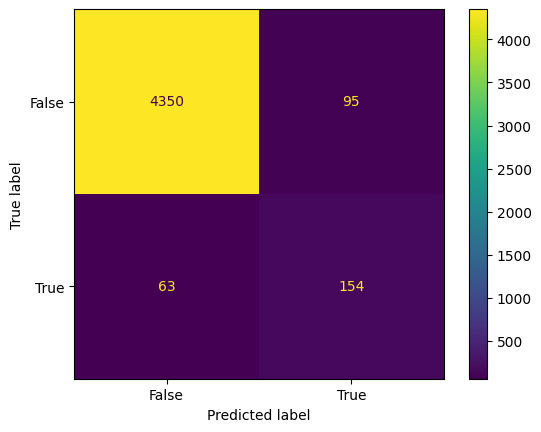
\includegraphics[width=0.4\textwidth]{BayesMatrix}}
\subfloat{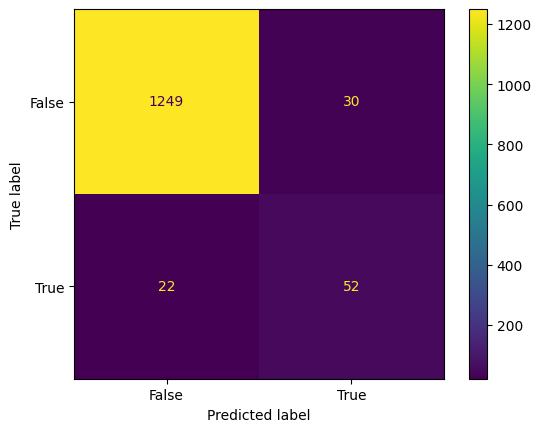
\includegraphics[width=0.4\textwidth]{BayesMatrixResults}}
\caption{A la izquierda se observa la matriz de confusión de entrenamiento del mejor modelo bayesiano obtenido según validación cruzada. Es notable la cantidad de falsos negativos, podrían ser demasiados en entornos reales donde esta equivocación puede incurrir en algún riesgo.
Observamos un comportamiento similar en la evaluación final (derecha). }
\label{fig:BayesMatrix}
\end{figure}


\section{Árboles de clasificación (Miguel García)}
\section{Gradient Boosting (Miguel García)}
\section{Stacking (Brian Sena)}
El \textit{Stacking} (apilamiento) es una técnica de aprendizaje automático que combina las predicciones de múltiples modelos base para construir un modelo final más robusto y preciso. 
A diferencia de otros métodos de ensamblado, en el \textit{Stacking} se utiliza un modelo de nivel superior, conocido como meta-modelo, que aprende a combinar las predicciones de los modelos base.
El \textit{Stacking} es particularmente útil cuando diferentes modelos base capturan distintos patrones en los datos, ya que el meta-modelo puede aprovechar la diversidad para mejorar el rendimiento global. 
\subsection{Asunciones de Stacking}
\begin{itemize}
    \item \textbf{Diversidad de los modelos base}: El stacking asume que los modelos base son suficientemente diversos y que cada uno aporta información única sobre los datos. Si los modelos base son demasiado similares, su combinación puede no aportar mejoras significativas.
    \item \textbf{Relación entre modelos base y meta-modelo}: El meta-modelo debe ser lo suficientemente flexible como para aprender a interpretar las predicciones de los modelos base. Esto incluye identificar cuáles son más confiables para ciertas regiones del espacio de características.
    \item \textbf{Distribución de clases equilibrada}: Si los datos están desbalanceados, tanto los modelos base como el meta-modelo pueden sesgar sus predicciones hacia la clase mayoritaria, reduciendo la capacidad de detectar la clase minoritaria.
    \item \textbf{Independencia de errores}: Aunque los modelos base pueden cometer errores, se espera que estos errores no estén perfectamente correlacionados entre ellos, de modo que el meta-modelo pueda mitigarlos al combinar las predicciones.
\end{itemize}
\subsection{Preprocesamiento}
Se ha utilizado como modelo base aquellos implementados en diferentes secciones. Es decir, máquina de soporte vectorial (SVM por sus siglas en inglés), árbol de decisión y clasificador bayesiano simples. 
Los modelos son suficientemente distintos como para asumir que cada uno aportará información relevante para la resolución del problema. El árbol de decisión es capaz de modelar no-linealidades, la máquina de soporte una 
frontera de decisión y, por último, el clasificador bayesiano las probabilidades de las clases.
Para ello, se ha creado un pipeline específico para cada modelo para preprocesar los datos conforme sus necesidades. Por ejemplo, en el caso de las máquinas de soporte vectorial, escalar los datos. 
No se dispone de variables categóricas ni valores faltantes, por lo cuál lo único que difiere es el la presencia (o no) del escalado y la posible selección de variables.
Para el caso de los árboles no se ha realizado ningún paso previo. Para el caso de SVM, se ha añadido un escalado como paso previo. 
Para experimentar con el ajuste de la distribución de las clases, al igual que en el clasificador bayesiano, se ha hecho experimentos con ``\textit{CondensedNearestNeighbour} (CNN)'' y ``\textit{SMOTE + TomekLinks} (SMOTETomek)''.
Aunque la idea es modelar diferentes características en cada modelo, y que sus errores sean independientes, se ha realizado una prueba adicional utilizando los mejores parámetros obtenidos en las experimentaciones previas de cada modelo individual.
\subsection{Detalles de experimentación y resultados} 
Se ha hecho uso de las mismas librerías definidas en la Sección~\ref{sec:ExpBayes}. Los mismos 4 pliegues de validación cruzada y las métricas de la Sección~\ref{sec:Metricas}.
Los hiperparámetros que se buscan para cada modelo serán similares a los que se han utilizado en las diferentes secciones.
Para el modelo de soporte vectorial se buscarán los valores de regularización (C) entre 0.1, 1 y 10.
Para el árbol de decisión se ha experimentado tanto con criterio de corte (ct) de ``gini'' y ``entropía''. También se estudia profundidad ilimitada frente a máxima profundidad equivalente a 10.
Los resultados se recogen en la Tabla~\ref{tab:StackingResults} y la matriz de confusión de entrenamiento en la Figura~\ref{fig:StackingMatrix}.

\begin{table}[!ht]
    \centering
    \begin{tabular}{llc}
        \hline
        \textbf{Modelo} & \textbf{Parámetros} &\textbf{F1 Promedio} \\\hline
        Stacking & C=10, $\alpha$ = $1e^{-9}$, ct=``entropía''& 0.9376\\ 
        Stacking + SMOTE & C=10, $\alpha$ = $1e^{-9}$, ct=``gini''& 0.9309 \\ 
        Stacking + CNN & C=10, $\alpha$ = $1e^{-9}$, ct=``gini'' & 0.8726 \\ 
        Stacking + OPT & C=10, $\alpha$ = $1e^{-9}$, ct=``entropía''& \textbf{0.9438} \\ 
        \hline
    \end{tabular}
    \caption{Resultados promedios obtenidos sobre las diferentes combinaciones de modelos de apilamiento. El término OPT hace alusión a un modelo de apilamiento en el cuál cada modelo base está utilizando la mejor configuración posible (El bayesiano se entrena con un submuestreo por CNN y características seleccionadas por chi-cuadrado). Se observa una posible saturación del conjunto de entrenamiento.} 
    \label{tab:StackingResults}
\end{table}

Los resultados del mejor modelo sobre el conjunto final de evaluación se recogen en la Tabla~\ref{tab:StackingFinalResults} y su matriz de confusión en la Figura~\ref{fig:StackingMatrix}.
Utilizar este conjunto de modelos y un meta-modelo para modelar la iteracción entre ellos resulta ser muy eficaz para la resolución de este problema.

\begin{table}[!ht]
    \centering
    \begin{tabular}{lcccc}
        \hline
        \textbf{Modelo} & \textbf{Parámetros} &\textbf{Precisión} &\textbf{Sensibilidad} &\textbf{F1} \\\hline
        Stacking + OPT & C=10, $\alpha$=$1e^{-9}$, ct=``entropía'' & 0.9889 & 0.9387 & 0.9623\\ 
        \hline
    \end{tabular}
    \caption{Resultados finales obtenidos en el conjunto de test con el mejor modelo de apilamiento.}
    \label{tab:StackingFinalResults}
\end{table}

\begin{figure}[!ht]
\centering
\subfloat{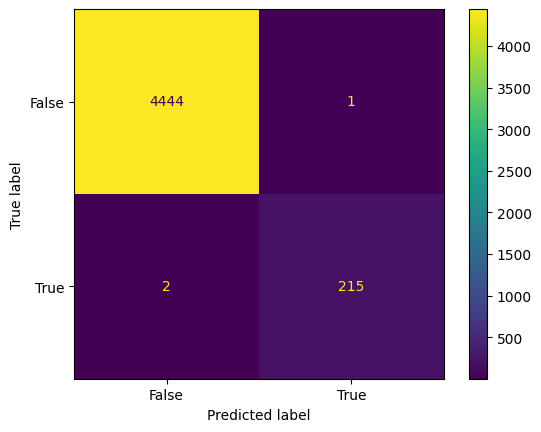
\includegraphics[width=0.4\textwidth]{StackingMatrix}}
\subfloat{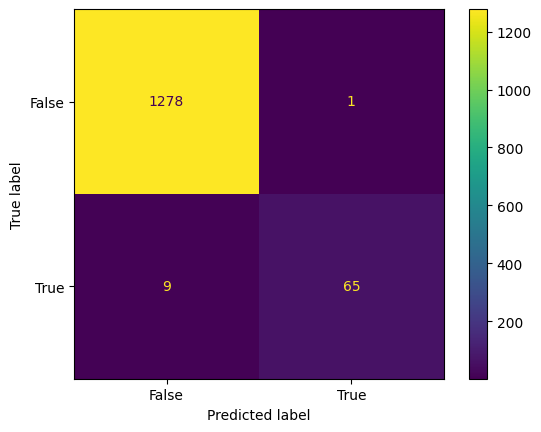
\includegraphics[width=0.4\textwidth]{StackingMatrixResults}}
\caption{A la izquierda se observa la matriz de confusión de entrenamiento del mejor modelo de apilamiento obtenido según validación cruzada. Observamos un rendimiento de casi el 100\% sobre el conjunto de entrenamiento.
En el conjunto final de evaluación presentamos una cantidad razonable de falsos negativos.}
\label{fig:StackingMatrix}
\end{figure}


\section{Regresión Logística (Álvaro Santana)}
\section{Bagging (Ana Fuentes)}

Por útlimo, se han trabajado con diferentes técnicas de Bagging para la clasificación de este dataset. En concreto, se han implementado tres ensembles; Random Forest, ExtraTrees y Random subspaces. Para estos algoritmos no es necesario escalar los datos, por lo que no se ha hecho ningún preprocesameinto adicional.

\subsection{Random Forest}
Random Forest es un ensemble de árboles de decisión entrenados con subconjuntos de datos obtenidos mediante muestreo con reemplazo (bootstrap).\\
Estos árboles se construyen de forma independiente y las predicciones para clasificación se combinan mediante el voto mayoritario.\\
Para este modelo, se han tomado los siguientes hiperparámetros:
\begin{itemize}
    \item n\_estimators: este parámetro es el número de árboles.
    \item max\_depth: este hace referencia a la profundidad máxima de los árboles.
    \item min\_samples\_split: este es el número mínimo de muestras requeridas para dividir un nodo.
    \item min\_samples\_leaf: es el número mínimo de muestras en una hoja.
\end{itemize}

De esta manera, se han generado 324 combinaciones y se han entrenado para obtener el mejor modelo. Así pues, la mejor combinación se ha mostrado en la Tabla \ref{tab:hiper_RF}.
\begin{table}[H]
    \centering
    \begin{tabular}{cccc}
    \hline
    \textbf{n\_estimators} &  \textbf{max\_depth} & \textbf{min\_samples\_split} & \textbf{min\_samples\_leaf} \\ \hline
    100 & None & 2 & 4 \\ \hline
    \end{tabular}
    \caption{Resultados de los mejores hiperparámetros obtenidos tras entrenar el modelo Random Forest.}
    \label{tab:hiper_RF}
\end{table}

Tras haber entrenado y haber obtenido la mejor combinación de los hiperparámetros, se ha evaluado el modelo con el conjunto de prueba, obteniéndose los resultados de la clasificación de la Tabla \ref{tab:res-RF}. También se ha mostrado la matriz de confusión en la Tabla \ref{tab:confusion-RF}.
\begin{table}[H]
    \centering
    \begin{tabular}{ccccc}
    \hline
    \textbf{Clase} & \textbf{Precisión} & \textbf{Recall} & \textbf{F1-score} & \textbf{Soporte} \\ \hline
    False & 1.00 & 1.00 & 1.00 & 1279 \\ 
    True & 0.96 & 0.95 & 0.95 & 74 \\ 
    macro avg & 0.98 & 0.97 & 0.97 & 1353 \\ 
    weighted avg & 0.99 & 0.99 & 0.99 & 1353 \\ \hline
    \end{tabular}
    \caption{Informe de clasificación tras la evaluación del mejor modelo de Random Forest para el conjunto de prueba.}
    \label{tab:res-RF}
\end{table}

\begin{table}[H]
    \centering
    \begin{tabular}{|cc|}
    \hline
    1276 & 3 \\
    4 & 70 \\ \hline
    \end{tabular}
    \caption{Mattriz de confusión obtenida para el ensemble Random Forest.}
    \label{tab:confusion-RF}
\end{table}

Analizando los resultados de estas Tablas, se puede comprobar que hay un mejor equilibrio entre la precisión y el recall. Por otro lado, aunque los resultados son notablemnte buenos, para la clase ``True'' (es anomalía), se hann obtenido peores resultados comparados con los arrojados para la clase ``False'' (no es anomalía), lo que puede explicarse debido al desbalanceo presente entre estas clases (74 frente a 1279).

Se puede concluir entonces que este modelo es muy buena opción para tratar estos datos debido a la robustez de este ensembble.

\subsection{ExtraTrees}
El ensemble ExtraTrees (Extremely Randomized Trees) es similar al algoritmo Random Forest, pero introduce más aleatoriedad durante la construcción de los árboles al seleccionar divisiones aleatorias en las características.\\
En  este caso, los hhiperparámetros que se han estudiado han sido los mismos que para el caso de Random Forest, pero en esta ocasión la aleatoriedad en las divisiones es mayor. Una vez entrenadas las 64 combinaciones posbiles, los mejores parámetros se han reflejado en la Tabla \ref{tab:hiper-ET}.
\begin{table}[H]
    \centering
    \begin{tabular}{cccc}
    \hline
    \textbf{n\_estimators} &  \textbf{max\_depth} & \textbf{min\_samples\_split} & \textbf{min\_samples\_leaf} \\ \hline
    200 & 10 & 5 & 2 \\ \hline
    \end{tabular}
    \caption{Resultados de los mejores hiperparámetros obtenidos tras entrenar el modelo ExtraTrees.}
    \label{tab:hiper-ET}
\end{table}

Con este modelo ya entrenado, se ha evaluado con el dataset de test, mostrando en la Tabla \ref{tab:res-ET} el reporte de clasificación y en la Tabla \ref{tab:confusion-ET} la matriz de confusión.
\begin{table}[H]
    \centering
    \begin{tabular}{ccccc}
    \hline
    \textbf{Clase} & \textbf{Precisión} & \textbf{Recall} & \textbf{F1-score} & \textbf{Soporte} \\ \hline
    False & 1.00 & 1.00 & 1.00 & 1279 \\ 
    True & 0.97 & 0.93 & 0.95 &  74 \\ 
     macro avg & 0.98 & 0.97 & 0.97 & 1353 \\ 
    weighted avg  & 0.99 & 0.99 & 0.99 & 1353 \\ \hline
    \end{tabular}
    \caption{Informe de clasificación tras la evaluación del mejor modelo de ExtraTrees para el conjunto de prueba.}
    \label{tab:res-ET}
\end{table}

\begin{table}[H]
    \centering
    \begin{tabular}{|cc|}
    \hline
    1277 & 2 \\
    5 & 69 \\ \hline
    \end{tabular}
    \caption{Matriz de confusión generada tras la evaluación del ExtraTrees.}
    \label{tab:confusion-ET}
\end{table}

Observando estas dos Tablas, se puede comprobar que este modelo arroja resultados muy similares a Random Forest, pero con un enfoque más aleatorio en la selección de divisiones. En la matriz de confusión se puede observar que para la clase ``False'' ha fallado menos que el ensemble Random Forest, pero para la clase ``True'' ha fallado más el ensemble ExtraTrees. De igual modo, este modelo ha demostrado presentar un alto rendimiento para este dataset.

\subsection{Random Subspaces}
Finalmente, se ha implementado el modelo de ensemble RRandom Subspaces. Este algoritmo es una técnica que construye un ensemble de clasificadores base (en este caso, se ha utilizado un ensemble de árboles de decisión) entrenados en subconjuntos aleatorios de características.\\
Los hiperparámetros para este modelo son los siguientes:
\begin{itemize}
    \item n\_estimators: este indica el número de clasificadores base en el ensemble.
    \item max\_features: este término indica la proporción de características seleccionadas para cada clasificador.
    \item estimator\_max\_depth: es la profundidad máxima de cada árbol de decisión.
\end{itemize}

En esta ocaasión, se han generado 108 combinaciones, por lo que después de entrenar los modelos generados ha resultado que los mejores parámetros para este conjunto de datos han sido los mostrados en la Tabla \ref{tab:hiper-RS}.
\begin{table}[H]
    \centering
    \begin{tabular}{ccc}
    \hline
    \textbf{n\_estimators} &  \textbf{max\_features} & \textbf{estimator\_max\_depth } \\ \hline
    50 & 0.5 & None \\ \hline
    \end{tabular}
    \caption{Resultados de los mejores hiperparámetros obtenidos tras entrenar el modelo Random Subspaces.}
    \label{tab:hiper-RS}
\end{table}

A continuación, se ha evaluado este algoritmo con el conjunto de prueba, obteniéndose los resultados de la Tabla \ref{tab:res-RS} y la matriz de confusión de la Tabla \ref{tab:confusion-RS}. 
\begin{table}[H]
    \centering
    \begin{tabular}{ccccc}
    \hline
    \textbf{Clase} & \textbf{Precisión} & \textbf{Recall} & \textbf{F1-score} & \textbf{Soporte} \\ \hline
    False & 1.00& 1.00 &  1.00 & 1279 \\ 
    True & 0.96 & 0.92 & 0.94 &  74 \\ 
    macro avg &  0.98 & 0.96 & 0.97 & 1353 \\ 
    weighted avg & 0.99 &  0.99 & 0.99 & 1353 \\ 
    \hline
    \end{tabular}
    \caption{Informe de clasificación tras la evaluación del mejor modelo de Random Subspaces para el conjunto de prueba}
    \label{tab:res-RS}
\end{table}

\begin{table}[H]
    \centering
    \begin{tabular}{|cc|}
    \hline
    1276 & 3 \\
    6 & 68 \\ \hline 
    \end{tabular}
    \caption{Matriz de confusión para el modelo Random Subspaces.}
    \label{tab:confusion-RS}
\end{table}

Aunque este ensemble también arroja unos resultados excelentes, para la clase ``True'' ha obtenidos los peores resultados para la precisión y el recall, comparados con los dos anteriores; esto se ha podido comprobar también en la matriz de confusión. El empeoramiento de la precisión en esta clase puede deberse a la selección aleatoria de características.

Finalmente, los modelos Random Forest y ExtraTrees son más confiables que este último algoritmo, puesto que tienen un valor de F1-score del 95\%, superior al F1-score que se ha obtenido en el modelo Random Subspaces.

\printbibliography
\end{document}
